\documentclass{esannV2}
\usepackage{graphicx}
\usepackage[utf8]{inputenc}
\usepackage{amssymb,amsmath,amsthm,array,booktabs}
\usepackage{url}
\usepackage{adjustbox}
\usepackage{placeins}
\usepackage{tikz}
\usetikzlibrary{arrows.meta,shapes.geometric}
\voffset 0 cm \hoffset -0.14 cm
% Supplementary material for the 6-page ESANN paper (main.tex). It carries the complete content of the
% full draft research/paper-acm-rpt/v3/main.tex (all sections, tables, figures and appendices),
% converted to the ESANN template. Generated by make_supplementary.py from supp_front.tex + the full draft; edit those, not supplementary.tex.
\newtheorem{proposition}{Proposition}
\emergencystretch=3em
\setcounter{topnumber}{3}\setcounter{totalnumber}{5}
\renewcommand{\topfraction}{0.93}\renewcommand{\textfraction}{0.06}\renewcommand{\floatpagefraction}{0.8}
\setlength{\tabcolsep}{3.5pt}
\renewcommand{\thesection}{S\arabic{section}}
\newcommand{\OSC}{\textsc{osc}}
\newcommand{\RPT}{\textsc{elpis}}
\newcommand{\Rone}{\textsc{elpis-r}}
\newcommand{\AUTO}{\textsc{elpis-cal}}
\newcommand{\AUTOD}{\textsc{elpis-g}}
\newcommand{\EJ}{\textsc{elpis-j}}
\newcommand{\EJG}{\textsc{elpis-jg}}
\newcommand{\s}{$^{\ast}$}
\begin{document}
\title{Supplementary Material:\\ Error-Labelled Perturbation Training for Selective RUL Prediction under Sensor Faults}
\author{AUTHOR-1$^1$ and AUTHOR-2$^2$
\vspace{.3cm}\\
1- INSTITUTION-1 - DEPARTMENT \\ ADDRESS - COUNTRY
\vspace{.1cm}\\
2- INSTITUTION-2 - DEPARTMENT \\ ADDRESS - COUNTRY\\
}
\maketitle
\noindent\fbox{\parbox{0.97\textwidth}{\footnotesize This supplement contains the complete extended version of the paper: every section, table, figure and appendix of the full draft, so that no result is lost in the 6-page version. Sections are numbered S1, S2, \dots; tables and figures are numbered independently of the main paper. Draft --- not ready for submission.}}

\begin{abstract}\textit{(Extended abstract.)} 
An optimistic remaining-useful-life (RUL) prediction can let an asset run past its safe window. Selective prediction can abstain, but dispersion- and novelty-based abstention fails under sensor faults: a fault shifts all ensemble members together, so they agree while the prediction turns optimistic. We train a one-sided selector, which estimates the probability of an optimistic error, on extra windows whose random channel subsets receive large perturbations, each labelled by whether the fixed predictor actually becomes optimistic on it (\RPT). Labelling the same windows as outliers instead is 1.6--5.2 points worse, and per-channel sensitivity features of the predictor do not replace them. This error-labelled perturbation training acts as a regulariser for scarce selector data: its gain grows as selector units become fewer, and it hurts on real hard-drive failures, where selector data are plentiful. A calibration-only gate (\AUTOD), pre-registered after the hard-drive results, decides per deployment whether to use it. In the last three of ten pre-registered confirmatory rounds (30 fresh seeds each, seed-level tests), \AUTOD{} lowered the optimistic-error rate at 90\% coverage under six unseen fault types on all four benchmark families (by 0.29--1.04 points, in every one of 20 disjoint sets of test units) and left hard drives unchanged; it lowered the fault-induced excess on the windows a fault changes on C-MAPSS, N-CMAPSS and batteries (by 0.71--2.04 points); and on three families it also beat the unperturbed selector on top of our JEPA-pretrained predictor \EJ{} (by 0.81--1.14 points). On implausible jumps in the raw battery measurements, which double the predictor's optimistic rate, the optimistic rate among accepted jump windows was about 3.5 times lower, found in an exploratory analysis and replicated in a pre-registered one. The gains are modest in absolute terms, and the evidence is on injected faults apart from the battery jumps.
\end{abstract}

\section{Introduction}
In predictive maintenance, the prognostics module of a monitoring system or digital twin turns sensor streams into remaining-useful-life (RUL) estimates~\cite{saxena2008damage}, and these estimates trigger inspection or replacement. The two error directions are not equally costly: an early prediction wastes some useful life, whereas an optimistic one can let an asset run past its safe window. Selective prediction~\cite{chow1970optimum,geifman2017selective,zaoui2020regression,jiang2020riskcontrolled} lets the model abstain on doubtful inputs and route them to inspection, so which inputs to reject is a safety decision.

The usual abstention signals fail exactly when sensors fail. Most measure predictive dispersion: ensemble spread~\cite{lakshminarayanan2017simple}, MC dropout~\cite{gal2016dropout}, Laplace approximations~\cite{daxberger2021laplace} or evidential uncertainty~\cite{amini2020deep}; others flag unusual inputs~\cite{lee2018simple,sun2022out,liu2008isolation}. A biased or stuck sensor shifts every ensemble member in the same direction, so the members agree while the prediction becomes optimistic (Prop.~\ref{prop:gauss}, measured in Sec.~\ref{sec:theory}), and an input can look unusual without harming the prediction, or look normal while harming it. A \emph{one-sided} selector that directly estimates the probability of the costly event, $\eta(x)=P(\hat y-y>\delta\mid x)$, avoids both problems, but it must learn what an optimistic error looks like from the shifts available in training and extrapolate to faults it has never seen.

Our idea is to label perturbed data by the predictor's own error rather than as anomalous. We add windows in which random channel subsets receive large perturbations and label each by whether the fixed predictor actually becomes optimistic on it (\textbf{E}rror-\textbf{L}abelled \textbf{P}erturbations for \textbf{I}nspection-aware \textbf{S}election, \RPT), in the spirit of domain randomization~\cite{tobin2017domain}. Labelling the same windows as outliers, as outlier exposure would, is clearly worse, and giving the selector the predictor's per-channel sensitivities instead of the perturbed copies does not help: the selector learns where large deviations make the predictor optimistic.

We also characterise when this works, which turns out to matter as much as the method. Error-labelled perturbation training acts as a regulariser for scarce selector data: its gain grows as selector units become fewer, and on real hard-drive failures, with hundreds of selector units and perturbations that do not make the predictor optimistic, it hurts (Fig.~\ref{fig:lc}). A diagnostic computed on calibration data alone, whether perturbing the deployment's own clean windows raises the predictor's optimistic rate, decides per deployment whether to use the scheme (\AUTOD). It is the method we pre-registered and confirmed, but a direct test shows that the harm on hard drives comes from the size of the selector set rather than from the sign of the diagnostic, so in practice the simplest guide is to use perturbation training when selector data are scarce.

The evidence comes from ten pre-registered confirmatory rounds with $\alpha$-spending on four benchmark families and real hard-drive failures. In round 8, on 30 fresh seeds with rotated test units and seed-level tests, \AUTOD{} lowered the optimistic-error rate under six unseen fault types on all four benchmark families, in every one of 20 disjoint sets of test units, with lower average risk at every coverage from 50 to 95\% (post hoc), and it never switched on hard drives, which it therefore left unchanged; round 9 confirmed the fault-specific part of the gain, and round 10 confirmed the gain on top of our JEPA-pretrained, fault-aware predictor \EJ. In an exploratory analysis of implausible jumps in the raw battery measurements, which double the predictor's optimistic rate, it also accepted far fewer optimistic windows.

\paragraph{Contributions.}
\begin{itemize}
\item \textbf{Method.} \RPT{} (Error-Labelled Perturbations for Inspection-aware Selection), error-labelled randomized perturbation training for one-sided RUL selectors, and a calibration-only gate (\AUTOD) that decides per deployment whether to apply it (Sec.~\ref{sec:method}). The labels, not the perturbations, drive the gain, and the scheme also improves other directional error estimators, so the contribution is a training scheme rather than a particular model (Sec.~\ref{sec:novelty}).
\item \textbf{When and why it works.} Dispersion fails under faults on our data; perturbation training lowers the estimation error rather than covering the faults, cannot be replaced by sensitivity features, and acts as a regulariser whose benefit shrinks with selector data and turns into harm on real hard drives (Sec.~\ref{sec:theory}, Sec.~\ref{sec:novelty}, Sec.~\ref{sec:hdd}).
\item \textbf{A pre-registered evaluation.} Methods were selected on development seeds by fixed rules and tested once on never-used seeds, with $\alpha$-spending over ten rounds and seed-level confirmations of the recommended method in the last three (Sec.~\ref{sec:protocol}).
\item \textbf{Controls and external tests.} Sixteen external baselines, held-out and all-channel fault types, physical faults on raw signals, outlier-exposure, volume and class-balance controls, a robust predictor, a third backbone, the fault-specific part of the gain, real hard-drive failures including untouched drive models, natural battery jumps, and deployment with thresholds fixed in advance (Sec.~\ref{sec:results}).
\end{itemize}

\FloatBarrier
\section{Related work}\label{sec:related}
\paragraph{Selective prediction and regression.} Abstention dates back to Chow's optimal reject rule~\cite{chow1970optimum}. For deep networks, selective classification~\cite{geifman2017selective}, learned selection heads~\cite{geifman2019selectivenet} and selective regression~\cite{zaoui2020regression,jiang2020riskcontrolled} rank inputs by a confidence score. Most scores measure dispersion or a symmetric confidence; we target the asymmetric event that matters for maintenance. Conformal risk control~\cite{angelopoulos2024conformal}, Learn-then-Test~\cite{angelopoulos2021ltt} and conformalized selective regression~\cite{sokol2026conformalized} turn any score into thresholds with finite-sample guarantees under exchangeability, and AUGRC~\cite{traub2024overcoming} has been proposed to evaluate selective classifiers; these are complementary to our scores, but their guarantees do not hold under the unseen fault shifts we study.

\paragraph{Uncertainty and out-of-distribution scores.} Ensembles~\cite{lakshminarayanan2017simple}, MC dropout~\cite{gal2016dropout}, Laplace~\cite{daxberger2021laplace}, evidential regression~\cite{amini2020deep} and test-time augmentation~\cite{wang2019aleatoric} estimate dispersion. Feature-space detectors~\cite{lee2018simple,sun2022out} and anomaly detectors~\cite{liu2008isolation} flag unusual inputs. Error predictors~\cite{corbiere2019addressing,kamath2020selective,yoo2019learning} and heteroscedastic models~\cite{nix1994estimating} are closest to our objective; we compare against all of these. Related lines of work predict a model's accuracy under shift from synthetic or unlabeled data. The closest in spirit is Schelter et al.~\cite{schelter2020learning}, who train a performance predictor on synthetically corrupted copies of held-out data to validate a black-box classifier's batch accuracy. Similarly, AutoEval regresses dataset-level accuracy on a meta-dataset of transformed sets~\cite{deng2021labels}; ATC~\cite{garg2022leveraging}, difference of confidences~\cite{guillory2021predicting} and ensemble disagreement~\cite{jiang2022assessing} estimate accuracy from unlabeled target data, motivated by the finding that uncertainty calibration degrades under shift~\cite{ovadia2019trust}; perturbing validation data before post-hoc calibration improves calibration under drift~\cite{tomani2021posthoc}; and OpenMix trains classifiers to reject transformed outliers for misclassification detection~\cite{zhu2023openmix}. These estimate aggregate (batch-level) accuracy or flag misclassifications in classification; we estimate a per-window, one-sided regression error under unseen input corruptions, and our controls show that labelling synthetic inputs as outliers, the OpenMix and outlier-exposure route, fails here (Sec.~\ref{sec:novelty}).

\paragraph{Sensor faults in prognostics.} Model-based fault detection exploits analytic redundancy between sensors~\cite{chow1984analytical,isermann2005model}. Robust uncertainty quantification for RUL with faulty sensors~\cite{wang2025robustuq} modifies the predictor. We keep the predictor fixed and learn when to trust it; Sec.~\ref{sec:robust} compares the two strategies.

\paragraph{Perturbation training, outlier exposure and domain randomization.} Training with input noise regularises a network~\cite{bishop1995training}; corruption augmentation improves robustness to related corruptions~\cite{hendrycks2020augmix}, mostly to the extent that augmentations resemble the test corruptions~\cite{mintun2021interaction}. Outlier exposure~\cite{hendrycks2019deep} trains detectors to flag auxiliary outliers. Domain randomization~\cite{tobin2017domain} and domain generalization~\cite{zhou2023domain} train on synthetic variation so that unseen domains look familiar. Our setting differs in two ways: perturbations train the \emph{selector}, not the predictor, and each perturbed window is labelled by whether the fixed predictor actually becomes optimistic on it, not marked as an outlier. Sec.~\ref{sec:novelty} tests both differences directly.

\FloatBarrier
\section{Setting and motivating analysis}\label{sec:theory}
A fixed predictor $f$ (the mean of an $M{=}3$ ensemble) maps a window $x\in\mathbb R^{T\times d}$ to a RUL estimate; $E=f(X)-Y$ is its signed error. A score $s$ induces a selector $g_s$ that accepts the lowest scores up to coverage $c$, randomising ties so that coverage is exactly $c$. Its risk is $R(g)=\mathbb E[g\,\eta]/c$, the optimistic-error rate among accepted windows, with $\eta(x)=P(E>\delta\mid X=x)$. At every coverage, $g_\eta$ minimises $R$: it accepts the inputs least likely to produce the costly event, the selective analogue of the Neyman--Pearson lemma.

\begin{proposition}[Why dispersion fails under faults]\label{prop:gauss}
Let $E\mid X\sim\mathcal N(\mu(X),\sigma^2(X))$, so $\eta=\Phi((\mu-\delta)/\sigma)$. (i) If $\mu\equiv\mu_0<\delta$ is constant, ranking by $\sigma$ is optimal. (ii) Otherwise ranking by $\sigma$ has excess risk $\frac1c\{\mathbb E[(\eta-t_c)^+\mathbf 1\{\sigma<q_c\}]+\mathbb E[(t_c-\eta)^+\mathbf 1\{\sigma\ge q_c\}]\}$, where $t_c$ and $q_c$ are the $c$-quantiles of $\eta$ and $\sigma$; it is positive iff $P(\eta>t_c,\sigma<q_c)>0$.
\end{proposition}
\noindent Here $\sigma(x)$ is the conditional spread of the error, which ensemble spread only approximates. A fault that moves all members together changes the bias $\mu(x)$ much more than the spread, and so creates exactly the high-$\eta$, low-$\sigma$ inputs of (ii). We measured this premise. On the windows each fault actually alters, the median shift of the ensemble mean is 1.4--25 times the median change in ensemble spread, across 14 fault types and four families. Spread does carry some information, but on the turbofan families 11--40\% of the windows that a fault newly makes optimistic keep a spread below the clean median, so a median spread threshold would still accept them. Dispersion also loses on clean data, because it is symmetric: its fault-induced excess exceeds that of \OSC{} by 0.31--0.95 points, whereas its overall gap to \OSC{} is 1.06--7.30 points.

\begin{proposition}[A transfer bound for learned selectors]\label{prop:transfer}
Let $P$ be the training distribution of observed windows (clean, seen shifts and random perturbations) and $Q$ that of an unseen fault, and let $\hat\eta$ be any score estimated on $P$. Assume (A) \emph{invariance}: the law of $Y$ given the observed window $\tilde X=\tilde x$ is the same under $P$ and $Q$, so that $\eta_P=\eta_Q=\eta$ on the common support; and (B) \emph{support}: $Q_{\tilde X}\ll P_{\tilde X}$ with density ratio $w=dQ/dP$. If $\eta(\tilde X)$ and $\hat\eta(\tilde X)$ are continuous under $Q$, then at every coverage $c$
\[
R_Q(g_{\hat\eta})-R_Q(g_\eta)\;\le\;\frac1c\,\mathbb E_Q|\hat\eta-\eta|\;\le\;\frac1c\sqrt{1+\chi^2(Q\,\|\,P)}\;\big\|\hat\eta-\eta\big\|_{L_2(P)}.
\]
\end{proposition}
\noindent The proof is in Appendix~\ref{app:proof}. The selector only sees features $\phi(\tilde x)$, so in practice the bound applies to the distributions of $\phi$; it is vacuous when $Q$ is singular with respect to $P$ (for example, a stuck channel with exactly zero variance), and we use it as motivation rather than as a guarantee. The bound separates the two ways a selector can fail on an unseen fault. The first is \emph{estimation} error on the training distribution, $\|\hat\eta-\eta\|_{L_2(P)}$, which more training data and a good classifier reduce. The second is \emph{coverage} of the fault by the training distribution, $\chi^2(Q\|P)$, which only changing $P$ can reduce. Perturbation training can act on both terms. It spreads training mass over a larger neighbourhood of corrupted windows (coverage), and it supplies informative labels about how the fixed predictor responds to input deviations, which lowers the estimation error on clean and corrupted windows alike. We measured both terms post hoc on the round-4 runs. Estimation error, as the Brier score of $\hat\eta$ on held-out calibration windows under the seen shifts (on the same windows the irreducible part $\mathbb E[\eta(1-\eta)]$ is identical for both selectors, so Brier differences equal differences in $\|\hat\eta-\eta\|^2_{L_2}$), falls with \RPT{} by 16--36\% on N-CMAPSS, bearings and batteries (19--20 of 20 pairs) and is unchanged on C-MAPSS ($-1\%$); on the faulty test windows it falls by 9--27\% on C-MAPSS, N-CMAPSS and bearings. Coverage, estimated with a domain classifier between the selector's training features and the faulty test features, gives no consistent picture: the classifier separates the two slightly \emph{better} after adding the perturbations on N-CMAPSS and bearings (AUC $+0.02$ and $+0.04$) and slightly worse on C-MAPSS ($-0.02$), while the density-ratio estimate of $\chi^2(Q\|P)$ is too large and too dominated by clipped weights to be informative. The measurable effect of perturbation training is thus on the estimation term, on clean and faulty windows alike, except on C-MAPSS, where it appears only under faults; this matches the controls in Sec.~\ref{sec:novelty}: volume-matched copies do not help, and a selector trained on the evaluation faults themselves, which minimises their coverage term, is not better than \RPT. Assumption (A) is a covariate-shift assumption~\cite{shimodaira2000improving} on observed windows. It is strong for a training mixture, since $P(Y\mid\tilde x)$ depends on the mixing weights whenever corruption types are not identifiable from $\tilde x$, and it fails when a corrupted window coincides with a clean window from a different health state; no selector can separate those. The bound suggests four expectations, which we test in Sec.~\ref{sec:abl}. (H1) An unperturbed copy does not change $\chi^2$ and should not help. (H2) Perturbations must reach the deviation scale of real faults. (H3) Perturbing channel subsets should cover faults on some sensors better than dense small noise does. (H4) The waveform should matter only insofar as it changes which region of the selector's feature space is covered.

\FloatBarrier
\section{Method}\label{sec:method}
\begin{figure}[!htbp]
\centering
\resizebox{\textwidth}{!}{% ELPIS pipeline (TikZ). Requires tikz with arrows.meta and shapes.geometric. ESANN layout: panels re-arranged to ~13 cm width (same content as the ACM figure).
\begingroup
\definecolor{hdr}{RGB}{31,74,52}
\definecolor{pnl}{RGB}{248,249,247}
\definecolor{grn}{RGB}{226,236,226}
\definecolor{grnb}{RGB}{120,150,125}
\definecolor{org}{RGB}{252,232,205}
\definecolor{orgb}{RGB}{205,140,70}
\definecolor{blu}{RGB}{226,229,247}
\definecolor{blub}{RGB}{110,115,185}
\definecolor{sa}{RGB}{40,90,170}\definecolor{sb}{RGB}{235,130,30}\definecolor{sc}{RGB}{50,150,60}
\begin{tikzpicture}[x=1cm,y=1cm,font=\footnotesize,>={Stealth[length=2.2mm]},
  panel/.style={draw=black!35,dashed,rounded corners=4pt,fill=pnl},
  box/.style={draw=grnb,rounded corners=3pt,fill=grn,align=center,inner sep=3pt,line width=0.6pt},
  obox/.style={box,draw=orgb,fill=org},
  bbox/.style={box,draw=blub,fill=blu},
  dbox/.style={box,fill=hdr,draw=hdr,text=white,font=\footnotesize\bfseries},
  dia/.style={draw=grnb,fill=grn,diamond,aspect=2.1,align=center,inner sep=0.3pt,line width=0.6pt,font=\scriptsize},
  arr/.style={->,line width=0.8pt,draw=hdr},
  jarr/.style={->,line width=0.8pt,draw=blub,dashed},
  note/.style={font=\scriptsize\itshape,align=center,text=black!70}]
\newcommand{\phead}[4]{%
  \node[fill=hdr,text=white,font=\small\bfseries,rounded corners=5pt,anchor=west,inner xsep=6pt,inner ysep=3pt] at (#1+0.25,#2) {\hspace{4mm}#4};
  \node[circle,fill=hdr,draw=white,line width=1pt,text=white,font=\normalsize\bfseries,minimum size=6.5mm,inner sep=0pt] at (#1+0.25,#2) {#3};}
\newcommand{\sig}[5]{\draw[#4,line width=0.6pt,domain=0:#3,samples=40,smooth] plot (#1+\x,{#2+0.09*sin(\x*620+#5)+0.05*sin(\x*1500+2*#5)});}
\newcommand{\win}[3]{%
  \draw[black!60,line width=0.5pt] (#1,#2) rectangle ++(#3,1.05);
  \sig{#1+0.05}{#2+0.82}{#3-0.1}{sa}{0}\sig{#1+0.05}{#2+0.55}{#3-0.1}{sb}{70}\sig{#1+0.05}{#2+0.28}{#3-0.1}{sc}{150}}
% ---------------- panels (re-arranged) ----------------
\draw[panel] (0,0) rectangle (5.55,-4.05);
\draw[panel] (5.8,0) rectangle (13.0,-4.05);
\draw[panel] (0,-4.45) rectangle (5.55,-8.5);
\draw[panel,draw=grnb,solid,fill=grn!40] (5.8,-4.45) rectangle (13.0,-8.5);
\draw[panel] (0,-9.1) rectangle (13.0,-12.6);
\phead{0}{0}{1}{RUL predictor $f$ (fixed)}
\phead{5.8}{0}{2}{ELPIS perturbation training}
\phead{0}{-4.45}{3}{Selector training}
\phead{0}{-9.1}{4}{Per-deployment gates (calibration units only)}
% ---------------- panel 1 ----------------
\node[font=\scriptsize,align=center] at (1.0,-0.65) {sensor window\\$x\in\mathbb R^{T\times C}$};
\win{0.25}{-2.15}{1.2}
\node[box] (ens) at (3.0,-1.62) {default ensemble\\[-1pt]{\scriptsize (GRU / TCN)}};
\node[bbox,font=\scriptsize,text width=2.95cm] (ej) at (2.95,-3.2) {\textbf{ELPIS-J} (optional):\\JEPA-pretrained (EMA\\or SIGReg), frozen encoder};
\node[obox,minimum height=7mm] (fx) at (4.95,-1.62) {$f(x)$};
\draw[arr] (1.5,-1.62) -- (ens);
\draw[arr] (ens) -- (fx);
\draw[jarr] (ej.east) -| node[pos=0.72,right,font=\tiny,text=blub!80!black]{alternative} (fx.south);
\begin{scope}[shift={(0.6,0)}]
% ---------------- panel 2 ----------------
\node[font=\scriptsize,align=center] at (6.75,-0.65) {clean selector\\window $x$};
\win{6.15}{-2.15}{1.2}
\fill[green!45!black,opacity=0.25] (8.75,-1.32) rectangle (9.15,-0.42);
\win{8.3}{-1.47}{1.25}
\fill[green!45!black,opacity=0.25] (8.95,-2.87) rectangle (9.35,-1.97);
\win{8.3}{-3.02}{1.25}
\draw[arr] (7.4,-1.62) -- (8.25,-0.95);
\draw[arr] (7.4,-1.62) -- (8.25,-2.5);
\node[font=\scriptsize,align=center] at (10.65,-0.85) {perturbed\\copies $\tilde x$};
\node[note] at (10.8,-1.95) {$k\le C/2$ channels,\\amplitude $1$--$8\sigma$,\\smooth onset};
\node[obox,font=\scriptsize,text width=5.3cm] (lab) at (8.95,-3.52) {label $\tilde y=\mathbf 1\{f(\tilde x)-y>\delta\}$\\{\itshape = the predictor's own error, not ``perturbed''}};
\draw[arr,densely dotted] (fx.east) -- (5.08,-1.62) |- node[pos=0.78,above,font=\tiny]{$f$} (lab.west);
\end{scope}
\begin{scope}[shift={(-11.925,-4.45)}]
% ---------------- panel 3 ----------------
\node[box,font=\scriptsize,text width=2.25cm] (seen) at (13.35,-1.0) {seen shifts:\\clean / dropout / drift};
\node[obox,font=\scriptsize,text width=1.9cm] (cp) at (16.0,-1.0) {+ perturbed copies\\with labels $\tilde y$};
\node[box,text width=4.5cm] (hgb) at (14.7,-2.45) {gradient-boosting classifier\\$s(x)\approx P\big(f(x)-y>\delta\mid x\big)$};
\node[note] at (14.7,-3.55) {OSC: the same classifier\\trained without the copies};
\draw[arr] (seen) -- (seen|-hgb.north);
\draw[arr] (cp) -- (cp|-hgb.north);
\end{scope}
\begin{scope}[shift={(-6.3,0.15)}]
% ---------------- key points ----------------
\node[dbox,minimum width=5.4cm] at (15.725,-5.05) {Key points};
\foreach \y/\t in {-5.7/{one-sided: estimates\\$P(f(x)-y>\delta)$},
                   -6.4/{labels from the predictor's\\own errors, not outliers},
                   -7.05/{gates use calibration\\units only},
                   -7.7/{ELPIS-G confirmed in\\pre-registered rounds 7--10}}{
  \node[circle,fill=hdr,text=white,inner sep=0.8pt,font=\tiny] at (13.6,\y) {\checkmark};
  \node[anchor=west,align=left,font=\scriptsize] at (13.82,\y) {\t};}
\end{scope}
\begin{scope}[shift={(0,-4.5)}]
% ---------------- panel 4 ----------------
\node[box,font=\scriptsize,text width=2.2cm] (cal) at (1.45,-6.0) {calibration units\\of the deployment\\{\itshape (no test data)}};
\node[dia] (dg) at (4.45,-5.45) {ELPIS-G\\$D>0$\,?};
\node[note,anchor=north] at (4.45,-6.1) {$D$: rise in the optimistic\\rate when clean calibration\\windows are perturbed};
\node[bbox,font=\scriptsize,minimum width=2.1cm] (use1) at (7.4,-5.1) {selector ELPIS};
\node[box,font=\scriptsize,minimum width=2.1cm] (use0) at (7.4,-5.85) {selector OSC};
\node[dia,draw=blub,fill=blu] (jg) at (7.4,-7.3) {predictor gate:\\other $f$ better?};
\node[note,anchor=west] at (8.75,-7.62) {lower calibration risk of the\\selector chosen for each $f$};
\node[dbox,text width=2.95cm,align=center] (dep) at (11.4,-5.45) {accept the $c$ lowest\\$s(x)$, abstain on rest};
\draw[arr] (cal.east) -- ++(0.3,0) |- (dg.west);
\draw[arr] (dg.north east) -- node[above,font=\tiny,pos=0.4]{yes} (use1.west);
\draw[arr] (dg.south east) -- node[below,font=\tiny,pos=0.4]{no} (use0.west);
\draw[arr] (use1.east) -- ++(0.65,0) |- ([yshift=1.5mm]dep.west);
\draw[arr] (use0.east) -- ++(0.65,0) |- ([yshift=-1.5mm]dep.west);
\draw[jarr] (cal.south) |- (jg.west);
\draw[jarr] (jg.east) -- (11.4,-7.3) node[pos=0.5,above,font=\tiny,text=blub!80!black]{chosen $f$} -- (dep.south);
\end{scope}
% ---------------- row link: trained selector feeds the deployment ----------------
\draw[arr] (2.775,-8.5) -- (2.775,-8.68) -| (dep.north);
\end{tikzpicture}
\endgroup
}
\caption{Pipeline. (1) A fixed ensemble predictor $f$ maps a sensor window to a RUL estimate. (2) Error-labelled perturbation training: random channel subsets of clean selector windows receive large smooth perturbations, and each perturbed copy $\tilde x$ is labelled by whether the \emph{same} predictor becomes optimistic on it, $\mathbf 1\{f(\tilde x)-y>\delta\}$, not by whether it was perturbed. (3) A gradient-boosting classifier learns the optimistic-error probability $s(x)\approx P(f(x)-y>\delta\mid x)$ from these copies together with the seen shifts; \OSC{} is the same classifier trained without the perturbed copies. (4) For each deployment, \AUTOD{} (recommended) keeps \RPT{} only if perturbing the clean calibration windows raises the predictor's optimistic rate ($D>0$), otherwise \OSC; the earlier rule \AUTO{} (not shown) chose by calibration risk under the seen shifts. Optionally (dashed, exploratory), \EJ{} is a JEPA-pretrained predictor whose members can be pooled with the default ones, and \EJG{} chooses per deployment between the default and the pooled predictor by the calibration risk of the selector chosen for each. No test data are used, and the deployed selector accepts the windows with the lowest scores and abstains on the rest.}
\label{fig:method}
\end{figure}
\paragraph{One-sided selector (\OSC).} Fig.~\ref{fig:method} summarises the pipeline. \OSC{} is the selector of our earlier study (under review; reference anonymised); this paper builds on it. A histogram gradient-boosting classifier~\cite{pedregosa2011scikit} estimates $\eta(x)$ from features $\phi(x)$: the prediction, the ensemble spread, the elapsed time and per-channel window statistics. It is trained on \emph{selector} units, disjoint from the fit, calibration and evaluation units, under three shifts $\mathcal S=\{\text{clean},\text{dropout},\text{drift}\}$ (dropout: one random channel missing for 40 cycles; drift: one random channel ramping to $\pm2\sigma$ over 100 cycles), with labels $\mathbf 1\{f(x)-y>\delta\}$ and unit-normalised weights. Hyperparameters were fixed a priori: at most 7 leaves, at least 25 samples per leaf and $L_2$ penalty 2. We use gradient boosting because the selector input is heterogeneous tabular data (features on different scales with non-linear interactions), on which tree ensembles are typically stronger than neural networks~\cite{grinsztajn2022tree}; it also handles missing values and per-unit sample weights natively and trains quickly enough for the thousands of selectors in this study. The model and its hyperparameters were inherited from \OSC{} and not tuned here; the classifier study in Sec.~\ref{sec:clf} confirms the choice.

\paragraph{Error-labelled perturbation training (\RPT).} Each clean selector window receives $K$ perturbed copies $x+\Delta$:
\begin{itemize}
\item \emph{Channels.} $k\sim\mathcal U\{1,\dots,\max(1,\mathrm{round}(\rho n))\}$ of the $n$ value channels are chosen at random.
\item \emph{Perturbation.} On each chosen channel, $\Delta_{t,c}=A\,\varphi(t)$ in normalised units, with $A\sim\mathrm{LogUniform}(A_{\min},A_{\max})$ and a random smooth waveform $\varphi=\tilde\varphi/\max_t|\tilde\varphi|$, $\tilde\varphi(t)=\sum_{m=0}^{2}a_m\cos(\pi m t/T+b_m)$, $a_m\sim\mathcal N(0,1)$, $b_m\sim\mathcal U(0,2\pi)$.
\item \emph{Onset.} With probability 0.5, $\varphi(t)=0$ before a random onset.
\item \emph{Labels.} Each copy is labelled with the predictor's own error on it, $\mathbf 1\{f(x+\Delta)-y>\delta\}$.
\end{itemize}
The selector is the \OSC{} classifier trained on $\mathcal S\cup\{\text{rand}_1,\dots,\text{rand}_K\}$, with all other settings unchanged. The generator never uses the evaluation-fault generators. The \textbf{final configuration} (\RPT) uses $K=2$, $\rho=0.5$ and $A\in[1,8]$. The round-1 method (\Rone) used $K=1$, $\rho=0.2$ and $A\in[0.5,4]$, plus three features from a per-channel ridge reconstruction (analytic redundancy~\cite{chow1984analytical}): the prediction change after repairing suspicious channels, the number of suspicious channels and the maximum normalised residual.

\paragraph{Recommended: diagnostic-based selection (\AUTOD).} Perturbation training is not guaranteed to help: on our real hard-drive data it hurts (Sec.~\ref{sec:hdd}). \RPT{} can only learn from perturbations that actually produce optimistic errors. \AUTOD{} therefore perturbs the deployment's clean calibration windows with the \RPT{} generator (two copies, fresh seeds) and computes $D$, the increase in the fixed predictor's optimistic rate over the clean windows; it uses \RPT{} if $D>0$ and \OSC{} otherwise. $D$ uses calibration labels only, has no tuned threshold, and was proposed after the hard-drive results (Sec.~\ref{sec:hdd}). It met its pre-specified criterion in a separate round on fresh seeds and a fourth, untouched drive-model set (significant on C-MAPSS and N-CMAPSS), and was significant on all four benchmark families at the seed level on 30 further seeds.

\paragraph{Earlier rule: calibration-based selection (\AUTO).} Before \AUTOD, confirmatory rounds 4 and 5 used \AUTO{} (round 6 a margin variant of it), which trains both \OSC{} and \RPT{} and keeps, for each deployment, the one with the lower risk at 90\% matched coverage on the calibration units under the seen shifts $\mathcal S$ (ties go to \OSC). The choice uses neither perturbed data, which would favour \RPT, nor test data.

\FloatBarrier
\section{Experimental protocol}\label{sec:protocol}
\paragraph{Data and faults.}
\begin{itemize}
\item \emph{Datasets.} C-MAPSS FD001--FD004~\cite{saxena2008damage} (RUL capped at 125; held-out development engines, so the official test set is not reused); N-CMAPSS~\cite{arias2021ncmapss} (99 engines from nine sub-datasets, flight-averaged; official test units); 32 FEMTO~\cite{nectoux2012pronostia} and XJTU-SY~\cite{wang2020xjtusy} bearings (leave one operating condition out); 124 battery cells~\cite{severson2019battery}. Channels are the 14 informative C-MAPSS sensors, 19 N-CMAPSS signals (including flight conditions), 34 derived vibration features per bearing record, and 7 per-cycle battery features (capacities, resistance, temperatures, charge time). Windows span 30 cycles (C-MAPSS), 10 flights (N-CMAPSS) or 30 records (bearings, batteries). Splits are by physical unit (sizes in Appendix~\ref{app:splits}). Predictor RMSE is computed over all windows of the evaluation units, including early-life windows with capped targets; it is not comparable with the last-window RMSE on the official C-MAPSS test set reported in the RUL literature. On clean round-8 data it is 15.7 cycles on C-MAPSS and 0.145, 0.274, 0.093 and 0.294 (life fraction) on N-CMAPSS, bearings, batteries and hard drives. $\delta=20$ cycles on C-MAPSS; on the other families the target is the remaining-life fraction and $\delta=0.16$.
\item \emph{Unseen faults.} Six faults are injected per unit on three random channels over one interval (C-MAPSS: cycles $[t_0,t_0+60)$ with $t_0\sim\mathcal U\{40,\dots,80\}$; other families: 30\% of life starting at 20--40\%, where for hard drives life is measured on the 90-day capped horizon, so faults fall 27--72 days before failure), so windows outside the interval are unchanged: stuck-at, bias ($3\sigma$), noise ($2\sigma$), intermittent loss (50\% of records missing), spikes ($\pm6\sigma$ on 10\% of records) and gain ($\times1.5$).
\item \emph{Backbones.} Three-member GRU~\cite{cho2014learning} and TCN~\cite{bai2018empirical} ensembles retrained for every seed; the two backbones of a seed share its unit split. A confirmation round trains 240 ensembles (C-MAPSS 4 subsets, N-CMAPSS, 6 bearing folds and batteries, times 2 backbones and 10 seeds). A patch-based Transformer in the style of PatchTST~\cite{nie2023time} is a third backbone (Sec.~\ref{sec:backbone}).
\end{itemize}

\paragraph{Metrics.} The primary metric is the unit-weighted optimistic-error rate at 90\% \emph{matched} coverage, averaged over the six unseen faults. C-MAPSS subsets are averaged within each backbone--seed pair and bearing folds are weighted by their number of units. Secondary metrics are the pessimistic-error rate ($E<-\delta$), clean-data risk, risk--coverage curves, and risk and coverage under thresholds frozen on clean calibration units. All selectors rank the \emph{same} ensemble predictions. Throughout, ``points'' are percentage points, a ``pair'' is one backbone--seed combination (20 per family, from 10 independent unit splits), ``pairs improved'' counts strict improvements (identical selectors, as when \AUTO{} keeps \OSC, are ties), and the ``excess'' of a fault is risk under the fault minus risk on the same windows without it. The earlier \OSC{} study used clean-frozen thresholds as its primary metric; because frozen thresholds mix selector quality with the calibration shift between clean calibration units and faulty test units, this study fixed matched coverage as primary before any confirmatory round and reports frozen thresholds as secondary.

\paragraph{Development and confirmation.} Methods were developed on separate development seeds; every confirmatory round then tested a method fixed beforehand under the following protocol.
\begin{enumerate}
\item \emph{Development} on seeds 42--61 (40 backbone--seed pairs per family), all seen in earlier rounds.
\item \emph{Selection} of one primary method by a rule written before computing any candidate.
\item \emph{Confirmation} on 10 never-used seeds (20 pairs per family, 240 newly trained three-member ensembles). The test is a two-sided Wilcoxon signed-rank test per family with Holm correction. Round $j$ uses $\alpha_j=0.05/2^j$, so the family-wise error over all rounds is at most 0.05.
\end{enumerate}
\emph{Round 1} selected \Rone{} by its total difference to \OSC, and confirmed it on seeds 62--71 at $\alpha_1=0.025$. \emph{Round 2} selected the final \RPT{} by its total difference to the \emph{best} of \OSC{} and two directional error estimators on each family, preferring simpler candidates within a 0.02-point band. It tested \RPT{} against all three on seeds 72--81, with Holm correction over 12 tests at $\alpha_2=0.0125$. \emph{Round 3} replicated the unchanged \RPT{} on seeds 82--91 against the same comparators (Holm over 12, $\alpha_3=0.00625$). After the hard-drive validation, \emph{Round 4} tested \AUTO{} on fresh seeds 92--101 across all five families against the same three comparators (Holm over 15, $\alpha_4=0.003125$). \emph{Round 5} re-tested the unchanged \AUTO{} on fresh seeds 112--121 with a new primary endpoint, the fault-induced excess on the windows a fault actually changes (Sec.~\ref{sec:excess}), against \OSC{} on all five families (Holm over 5, $\alpha_5=0.0015625$). \emph{Round 6} tested a stricter switching rule for \AUTO{} (Sec.~\ref{sec:hdd}; Holm over 5, $\alpha_6=0.00078125$). \emph{Round 7} tested \AUTOD{} on fresh seeds 152--161 and a fourth drive-model set (Holm over 5, $\alpha_7=0.000390625$). \emph{Round 8} tested \AUTOD{} alone on 30 fresh seeds 162--191 with rotated test units, with the seed as the unit (Holm over 5, $\alpha_8=0.0001953125$). \emph{Round 9} tested the fault-induced excess on affected windows for \AUTOD{} alone on 30 fresh seeds 192--221 (seed level, Holm over 5, $\alpha_9=0.00009765625$). \emph{Round 10} tested \AUTOD{} against \OSC{} on the JEPA-pretrained predictor \EJ{} (Sec.~\ref{sec:checks}) on 30 fresh seeds 222--251 for C-MAPSS, batteries and bearings (seed level, Holm over 3, $\alpha_{10}=0.000048828125$). The family-wise error over all ten rounds is at most $0.049951171875$. Further analyses (baselines, stress tests, robust predictor, backbone, ablations) were pre-registered separately and could not change the method.

\FloatBarrier
\section{Results}\label{sec:results}

\begin{table}[!htbp]
\caption{Confirmatory results: pre-registered tests on never-used seeds within the $\alpha$-spending budget. Risk is the optimistic-error rate (\%) at 90\% matched coverage, averaged over six unseen faults; differences in percentage points (negative: better), with seeds (rounds 8--10, out of 30) or backbone--seed pairs (rounds 2--3, out of 20) improved and Holm-adjusted $p$. Rounds 1 and 4--7: Appendix Table~\ref{tab:history}.}
\label{tab:confirm}
\centering\footnotesize
\setlength{\tabcolsep}{4pt}
\begin{adjustbox}{max width=\textwidth}\begin{tabular}{lrrrr}
\toprule
 & C-MAPSS & N-CMAPSS & Bearings & Batteries\\
\midrule
\multicolumn{5}{l}{\textbf{Round 8:} \AUTOD{} vs.\ \OSC, seeds 162--191, $\alpha_8=0.0002$}\\
Risk, \OSC & 8.78 & 8.14 & 24.39 & 3.31\\
Risk, \AUTOD & \textbf{8.14} & \textbf{7.86} & \textbf{23.77} & \textbf{2.27}\\
Difference & $-0.64$ & $-0.29$ & $-0.62$ & $-1.04$\\
\quad seeds / $p$ & 30, 9e-9 & 30, 9e-9 & 27, 2e-7 & 30, 9e-9\\
\multicolumn{5}{l}{\quad Hard drives: $0.00$ ($D<0$ in every deployment, so \AUTOD{} = \OSC).}\\
\midrule
\multicolumn{5}{l}{\textbf{Round 9:} fault-induced excess on affected windows, seeds 192--221}\\
$\Delta$excess, \AUTOD{} $-$ \OSC & $-1.10$ & $-0.71$ & $-0.04$ & $-2.04$\\
\quad seeds / $p$ & 30, 9e-9 & 30, 9e-9 & 19, 0.25 & 30, 9e-9\\
\midrule
\multicolumn{5}{l}{\textbf{Round 10:} \AUTOD{} vs.\ \OSC{} on the pretrained predictor \EJ, seeds 222--251}\\
Difference & $-0.81$ & -- & $-1.03$ & $-1.14$\\
\quad seeds / $p$ & 30, 6e-9 & -- & 29, 6e-9 & 30, 6e-9\\
\midrule
\multicolumn{5}{l}{\textbf{Rounds 2 and 3:} \RPT{} vs.\ \OSC, seeds 72--81 and 82--91}\\
Round 2 & $-0.55$ & $-0.40$ & $-1.06$ & $-0.90$\\
\quad pairs / $p$ & 19, 4e-5 & 18, 7e-5 & 19, 4e-5 & 19, 4e-5\\
Round 3 (replication) & $-0.70$ & $-0.34$ & $-1.56$ & $-0.73$\\
\quad pairs / $p$ & 20, 2e-5 & 20, 2e-5 & 19, 3e-5 & 19, 3e-5\\
\bottomrule
\end{tabular}\end{adjustbox}
\end{table}
\begin{table}[!htbp]
\caption{Comparison with sixteen external baselines and one variant of our method on fresh seeds 72--81 (240 ensembles). Risk (\%) at 90\% matched coverage, averaged over six unseen faults; in parentheses, \RPT{} minus the baseline in points (negative: \RPT{} better). \s: significant after Holm over all 68 tests ($\alpha=0.05$). All selectors rank the same ensemble predictions. Bold: lowest risk in the column. \AUTOD{} switches to \RPT{} in 98--100\% of the C-MAPSS, N-CMAPSS and battery deployments and in 45\% of the bearing ones; it is below every external baseline on all four families.}
\label{tab:sota}
\centering\small
\begin{adjustbox}{max width=\textwidth}\begin{tabular}{llllll}
\toprule
Group & Baseline & C-MAPSS & N-CMAPSS & Bearings & Batteries\\
\midrule
Dispersion & Ensemble spread~\cite{lakshminarayanan2017simple} & 10.96 ($-1.99$\s) & 17.51 ($-7.70$\s) & 24.80 ($-2.82$\s) & 5.35 ($-1.97$\s)\\
 & MC dropout~\cite{gal2016dropout} & 11.42 ($-2.45$\s) & 17.95 ($-8.14$\s) & 24.61 ($-2.63$\s) & 5.78 ($-2.39$\s)\\
 & Deep ensemble, Gaussian NLL~\cite{lakshminarayanan2017simple} & 11.00 ($-2.02$\s) & 16.12 ($-6.31$\s) & 26.15 ($-4.17$\s) & 4.97 ($-1.58$\s)\\
 & Deep evidential regression~\cite{amini2020deep} & 11.29 ($-2.31$\s) & 16.06 ($-6.25$\s) & 26.28 ($-4.30$\s) & 5.08 ($-1.69$\s)\\
 & Last-layer Laplace~\cite{daxberger2021laplace} & 11.75 ($-2.78$\s) & 18.09 ($-8.28$\s) & 24.92 ($-2.94$\s) & 5.82 ($-2.43$\s)\\
 & Test-time augmentation~\cite{wang2019aleatoric} & 11.19 ($-2.21$\s) & 17.96 ($-8.16$\s) & 25.43 ($-3.45$\s) & 6.51 ($-3.12$\s)\\
OOD / anomaly & Mahalanobis distance~\cite{lee2018simple} & 11.67 ($-2.70$\s) & 16.85 ($-7.05$\s) & 25.68 ($-3.70$\s) & 4.99 ($-1.60$\s)\\
 & $k$-NN feature distance~\cite{sun2022out} & 11.99 ($-3.02$\s) & 17.97 ($-8.16$\s) & 25.47 ($-3.49$\s) & 5.62 ($-2.24$\s)\\
 & Isolation forest~\cite{liu2008isolation} & 12.94 ($-3.96$\s) & 17.97 ($-8.16$\s) & 24.82 ($-2.84$\s) & 5.77 ($-2.38$\s)\\
 & Analytic-redundancy residual~\cite{chow1984analytical} & 11.10 ($-2.13$\s) & 17.31 ($-7.50$\s) & 27.09 ($-5.11$\s) & 5.66 ($-2.27$\s)\\
Selective / interval & SelectiveNet~\cite{geifman2019selectivenet} & 12.54 ($-3.56$\s) & 17.37 ($-7.56$\s) & 26.52 ($-4.54$\s) & 5.48 ($-2.09$\s)\\
 & CQR lower bound~\cite{romano2019cqr} & 9.91 ($-0.94$\s) & 15.43 ($-5.62$\s) & 23.79 ($-1.81$\s) & 4.98 ($-1.59$\s)\\
Learned event / error & Symmetric classifier, $|E|>\delta$ (after~\cite{corbiere2019addressing,kamath2020selective}) & 12.47 ($-3.50$\s) & 14.54 ($-4.73$\s) & 26.07 ($-4.09$\s) & 4.88 ($-1.49$\s)\\
 & Perturbation detector (after~\cite{isermann2005model}) & 11.07 ($-2.10$\s) & 17.39 ($-7.58$\s) & 26.08 ($-4.10$\s) & 5.74 ($-2.36$\s)\\
 & Signed-error regression (after~\cite{yoo2019learning}) & 10.77 ($-1.79$\s) & 10.06 ($-0.25$\s) & 23.01 ($-1.03$\s) & 3.94 ($-0.55$\s)\\
 & Gaussian with learned bias (after~\cite{nix1994estimating}) & 10.12 ($-1.15$\s) & 10.06 ($-0.25$\s) & 23.46 ($-1.48$\s) & 3.93 ($-0.54$\s)\\
Augmentation & Sparse white-noise training (after~\cite{bishop1995training}; round-1 variant) & \textbf{8.93} ($+0.05$) & 9.98 ($-0.17$\s) & 22.85 ($-0.87$\s) & 3.87 ($-0.48$\s)\\
 & \OSC{} (one-sided classifier, ours) & 9.52 & 10.21 & 23.04 & 4.29\\
\midrule
 & \RPT{} (ours) & 8.97 & \textbf{9.81} & \textbf{21.98} & \textbf{3.39}\\
 & \AUTOD{} (ours, gated; recomputed on the same runs) & 8.98 & 9.81 & 22.55 & 3.37\\
\bottomrule
\end{tabular}\end{adjustbox}
\end{table}


\FloatBarrier
\subsection{Confirmatory results}
Rounds 1--5 and 7--10 met their pre-specified criterion (a significant gain over \OSC{} on at least one family, no significant loss, a mean difference of at most $+0.3$ points and a pessimistic rise of at most 1 point); round 6 did not. Table~\ref{tab:confirm} shows the final rounds. In round 8, \AUTOD{} lowered risk on every benchmark family by 0.29--1.04 points, in 27--30 of 30 seeds and in each of 20 disjoint sets of test units, with pessimistic rises of at most 0.47 points, and equalled \OSC{} on hard drives. Round 9 confirmed the fault-specific part of the gain and round 10 the gain on a stronger, pretrained predictor. The plain method \RPT{} was confirmed against \OSC{} and two directional estimators in rounds 2 and 3; it is better than \OSC{} in all 24 fault--family cells (Appendix Table~\ref{tab:fault}) and at every coverage (Fig.~\ref{fig:rc}). Seed- and unit-level uncertainty and the remaining headroom are analysed in Appendix~\ref{app:detail}. Appendix Table~\ref{tab:claims} lists the evidential status (confirmatory, pre-registered secondary or exploratory) of every claim.

\begin{table}[!htbp]
\caption{Ablation study (exploratory). Each row is a variant minus its reference, in points of risk at 90\% matched coverage under six unseen faults; positive means worse than the reference. \s: significant after Holm within the block. Top: reference \RPT, seeds 72--81 (sensitivity features: seeds 152--161). Middle: variants of the round-1 method \Rone{} minus \Rone, seeds 62--71. Bottom: selector model minus histogram gradient boosting (HGB) with the \OSC{} features, seeds 62--71.}
\label{tab:ablation}
\centering\footnotesize
\setlength{\tabcolsep}{3.5pt}
\begin{adjustbox}{max width=\textwidth}\begin{tabular}{lrrrr}
\toprule
 & C-MAPSS & N-CMAPSS & Bear. & Batt.\\
\midrule
\multicolumn{5}{l}{\emph{Labels and data, vs.\ \RPT}}\\
No perturbed copies (\OSC) & $+0.55$\s & $+0.40$\s & $+1.06$\s & $+0.90$\s\\
Two unperturbed copies & $+0.62$\s & $+0.42$\s & $+1.12$\s & $+1.00$\s\\
Two copies, tiny perturbations & $+0.57$\s & $+0.42$\s & $+1.23$\s & $+1.01$\s\\
\OSC, classes reweighted & $+0.53$\s & $+0.39$\s & $+1.08$\s & $+0.90$\s\\
Sensitivity features, no copies & $+0.53$\s & $+0.69$\s & $+0.74$\s & $+0.53$\s\\
Outlier-exposure labels~\cite{hendrycks2019deep} & $+1.63$\s & $+5.18$\s & $+2.33$\s & $+2.00$\s\\
Perturbation detector~\cite{isermann2005model} & $+2.49$\s & $+7.33$\s & $+2.73$\s & $+2.35$\s\\
Symmetric target $|E|>\delta$ & $+3.54$\s & $+4.52$\s & $+4.09$\s & $+1.17$\s\\
Oracle: train on the six test faults & $+0.15$ & $+0.09$ & $+1.04$ & $+0.16$\\
\midrule
\multicolumn{5}{l}{\emph{Generator, vs.\ \Rone}}\\
Unperturbed copy (H1) & $+0.26$\s & $+0.28$\s & $+0.40$ & $+0.40$\s\\
Small amplitude, $A\in[0.25,1]$ (H2) & $+0.21$\s & $+0.07$ & $+0.47$ & $+0.27$\s\\
Large amplitude, $A\in[2,8]$ (H2) & $-0.15$ & $-0.05$ & $-0.38$ & $-0.04$\\
Dense noise on all channels (H3) & $+0.23$\s & $+0.07$ & $+0.12$ & $+0.34$\s\\
One channel, $k=1$ (H3) & $0.00$ & $+0.08$\s & $+0.37$ & $0.00$\\
White-noise waveform (H4) & $+0.03$ & $-0.01$ & $+0.21$ & $+0.11$\\
No onset (H4) & $-0.06$ & $-0.02$ & $+0.13$ & $+0.06$\\
Two perturbed copies & $-0.15$\s & $-0.05$ & $+0.03$ & $-0.09$\\
\midrule
\multicolumn{5}{l}{\emph{Selector model, vs.\ HGB}}\\
Logistic regression~\cite{cox1958regression} & $+1.10$\s & $+2.45$\s & $+0.87$\s & $+0.15$\\
Random forest~\cite{breiman2001random} & $+0.70$\s & $+1.94$\s & $+0.44$ & $+0.37$\\
MLP (64, 64)~\cite{rumelhart1986learning} & $+1.65$\s & $+2.54$\s & $+1.23$\s & $+0.81$\s\\
\bottomrule
\end{tabular}\end{adjustbox}
\end{table}
\begin{table}[!htbp]
\caption{Is the gain robust? \RPT{} minus \OSC{} (points of risk at 90\% matched coverage; negative is better) under variations of the data, faults, threshold and predictor. \s: significant after Holm within its (pre-registered or exploratory) family; unmarked: descriptive. ``--'': not run.}
\label{tab:robustness}
\centering\footnotesize
\setlength{\tabcolsep}{3pt}
\resizebox{\textwidth}{!}{\begin{tabular}{lrrrr}
\toprule
Variation & C-MAPSS & N-CMAPSS & Bear. & Batt.\\
\midrule
Main setting (round 2) & $-0.55$\s & $-0.40$\s & $-1.06$\s & $-0.90$\s\\
Rotated test units & -- & $-0.25$\s & -- & $-1.09$\s\\
Four held-out fault types & $-0.47$\s & $-0.33$\s & $-1.05$\s & $-1.00$\s\\
Faults on all channels & $-0.60$\s & $-0.32$\s & $-1.13$\s & $-0.83$\s\\
Physical faults, raw signals & -- & -- & $-1.0$\s & --\\
Error threshold $0.5\delta$ & $-0.48$\s & $-0.17$\s & $-1.06$\s & $-0.77$\s\\
Error threshold $1.5\delta$ & $-0.60$\s & $-0.51$\s & $-1.36$\s & $-0.78$\s\\
Five-member ensembles & $-0.55$\s & $-0.44$\s & $-1.29$\s & $-1.02$\s\\
Patch-Transformer backbone & $-0.51$\s & $-0.49$\s & $-1.69$\s & $-0.84$\s\\
Larger GRU/TCN (\AUTOD) & $-0.62$ & -- & -- & --\\
Noise-trained predictor & $-0.43$ & $-0.24$ & $-1.28$ & $-0.82$\\
Pretrained \EJ{} (\AUTOD, round 10) & $-0.81$\s & -- & $-1.03$\s & $-1.14$\s\\
\bottomrule
\end{tabular}}
\end{table}
\begin{figure}[!htbp]
\centering
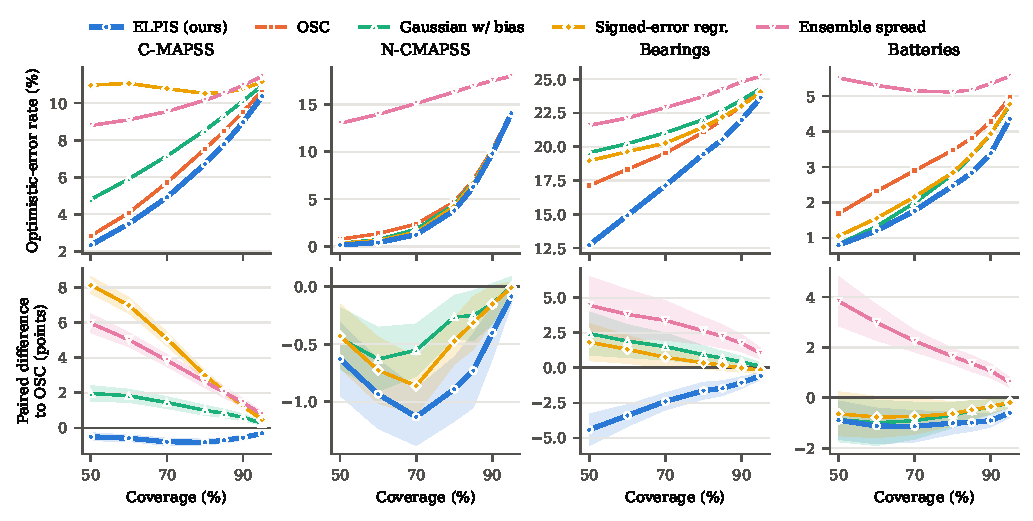
\includegraphics[width=\textwidth]{figures/risk_coverage.pdf}
\caption{Risk--coverage on round-2 seeds 72--81, averaged over six unseen faults. Top: optimistic-error rate among accepted windows (mean over 20 backbone--seed pairs). Bottom: paired difference to \OSC{} with $\pm1.96$ standard errors of the paired differences; below zero is better than \OSC{} (ensemble spread on N-CMAPSS, $+6$ to $+8$ points, is off scale). Baselines: \OSC{} (ours, without perturbations), Gaussian with learned bias (after~\cite{nix1994estimating}), signed-error regression (after~\cite{yoo2019learning}), ensemble spread~\cite{lakshminarayanan2017simple}. On C-MAPSS, the risk of signed-error regression stays at 10.5--11.1\% from 95\% down to 50\% coverage: the capped predictor's signed error is heavy-tailed, and the regression's most confident (most negative) predictions include windows that are in fact optimistic (an absolute or clipped loss does not change this; Sec.~\ref{sec:fair}).}
\label{fig:rc}
\end{figure}


\FloatBarrier
\subsection{Comparison with sixteen external baselines}\label{sec:sota}
Table~\ref{tab:sota} compares \RPT{} with sixteen external baselines on the same fresh seeds and ensemble predictions (a separately pre-registered family of 68 tests). \RPT{} is significantly better in 67 of 68 comparisons and never worse: by 0.9--8.3 points against the uncertainty, selective-prediction and anomaly scores, and by 0.25--1.79 points against the directional error estimators. Out-of-distribution and anomaly scores perform at the level of ensemble spread: detecting an unusual input is not the same as estimating whether the prediction is optimistic. Strengthened baselines (head models retrained on the same perturbations, better error regressions, fault detection and imputation, five-member ensembles; Appendix Table~\ref{tab:fair}), three post hoc baselines and a simplified fault-robust RUL system after RobustUQ~\cite{wang2025robustuq} do not change this, except that channel repair helps on bearings (Appendix~\ref{app:detail}). The one-sided selectors accept 2.5--4.8 points more pessimistic errors than the best symmetric score, the intended trade-off.

\FloatBarrier
\subsection{Ablation study}\label{sec:novelty}\label{sec:abl}\label{sec:clf}
Table~\ref{tab:ablation} isolates what the method needs.
\begin{itemize}
\item \emph{The labels are the method.} Labelling the same perturbed windows as outliers, or detecting them, is 1.6--7.3 points worse; extra data without informative perturbations, class reweighting or single-channel sensitivity features of the predictor leave risk at the level of \OSC.
\item \emph{Amplitude, not waveform.} Small amplitudes and dense noise are worse, larger amplitudes better; waveform and onset do not matter (H1--H4).
\item \emph{The target must be one-sided}, and gradient boosting is the strongest selector model; perturbation training helps every classifier (Appendix Table~\ref{tab:clf}).
\end{itemize}
Further controls (overlap between perturbations and faults, transfer to other directional estimators) are in Appendix~\ref{app:novelty}.

\FloatBarrier
\subsection{Robustness of the gain}\label{sec:stress}\label{sec:checks}\label{sec:backbone}\label{sec:robust}
The gain over \OSC{} holds on new test units, on fault types designed after the method was frozen, on faults outside the generator's range and on physical faults injected into raw bearing signals, at other error thresholds, with larger ensembles, a third backbone, a larger and a pretrained predictor (Table~\ref{tab:robustness}); across 13 severity and channel-count scenarios it is lower than \OSC{} in 50 of 52 cells (Fig.~\ref{fig:sev}). Making the predictor itself robust by training on the same perturbations helps on N-CMAPSS and batteries but hurts on C-MAPSS and bearings, and \RPT{} improves on \OSC{} with either predictor (Appendix Table~\ref{tab:robust}).

\FloatBarrier
\subsection{Gates and predictors}\label{sec:frozen}
\begin{table}[!htbp]
\caption{Gates and predictors. Top (round 8, seeds 162--191, mean over 30 seeds): each selector minus \OSC{} (points; negative is better) and the share of deployments in which \AUTOD{} uses \RPT. Bottom: risk (\%) of \AUTOD{} on three predictors, seeds 222--251, and \EJG{} against \AUTOD{} on the default predictor on fresh seeds 252--281 and, for bearings, 282--341 (exploratory). \EJ: JEPA-pretrained predictor; pooled: default plus \EJ{} members.}
\label{tab:deploy}
\centering\footnotesize
\setlength{\tabcolsep}{3pt}
\resizebox{\textwidth}{!}{\begin{tabular}{lrrrrr}
\toprule
 & C-MAPSS & N-CMAPSS & Bear. & Batt. & Drives\\
\midrule
\multicolumn{6}{l}{\emph{Selector gates, minus \OSC}}\\
\RPT{} always & $-0.64$ & $-0.29$ & $-1.43$ & $-1.04$ & $+0.41$\\
\AUTO{} (calibration risk) & $-0.46$ & $-0.22$ & $-0.90$ & $-1.03$ & $+0.03$\\
\AUTOD{} ($D>0$) & $-0.64$ & $-0.29$ & $-0.62$ & $-1.04$ & $0.00$\\
\quad uses \RPT & 100\% & 100\% & 42\% & 100\% & 0\%\\
\midrule
\multicolumn{6}{l}{\emph{Predictors, risk of \AUTOD{} (\%)}}\\
Default & 8.95 & -- & \textbf{22.50} & 2.35 & --\\
\EJ & 8.35 & -- & 24.49 & 1.90 & --\\
Pooled & \textbf{8.29} & -- & 22.86 & \textbf{1.68} & --\\
\multicolumn{6}{l}{\quad RMSE (default / \EJ{} / pooled): C-MAPSS 15.9 / 14.4 / 14.6; bearings .275 / .265 / .258;}\\
\multicolumn{6}{l}{\quad batteries .092 / .085 / .083.}\\
\midrule
\multicolumn{6}{l}{\emph{\EJG{} minus \AUTOD{} on the default predictor, seeds 252--281}}\\
Difference & $-0.58$ & -- & $-0.54$ & $-0.54$ & --\\
\quad seeds / $p$ & 29, $<$1e-4 & -- & 18, 0.13 & 30, $<$1e-4 & --\\
\multicolumn{6}{l}{\emph{Bearings replication, 60 further fresh seeds 282--341}}\\
Difference (90\% CI) & -- & -- & \multicolumn{3}{l}{$-0.56$ $[-0.97,-0.14]$; 28 of 60, $p=0.11$}\\
\bottomrule
\end{tabular}}
\end{table}
Plain \RPT{} hurts on real hard drives, and \AUTOD{} removes the harm while keeping the full gain on C-MAPSS, N-CMAPSS and batteries (Table~\ref{tab:deploy}, top; Sec.~\ref{sec:hdd}). On bearings, where $D$ is near zero, it keeps less than half of the gain. The pretrained predictor \EJ{} is more accurate and lowers risk on C-MAPSS and batteries but is more optimistic on bearings; pooling it with the default members, and choosing between the default and the pooled predictor per deployment by calibration risk (\EJG), lowered risk on C-MAPSS and batteries on fresh seeds and was non-inferior on bearings (exploratory). On bearings a pre-registered replication on 60 further fresh seeds gave a mean of $-0.56$ points (90\% interval $[-0.97,-0.14]$) but only 28 of 60 seeds improved (Wilcoxon $p=0.11$), so we report a tie: the average gain is carried by a minority of deployments, not a typical one. Frozen thresholds, maintenance simulations and expected cost are in Appendix~\ref{app:detail}: at every fixed coverage from 50 to 95\% \AUTOD{} accepts fewer optimistic errors than \OSC, and counting both error types it is cheaper already at equal costs.

\FloatBarrier
\subsection{How much of the gain is fault-specific?}\label{sec:excess}
\begin{table}[!htbp]
\caption{Fault-induced excess on the windows a fault actually changes (pre-registered secondary analysis on round-4 seeds 92--101, five families). Faults are injected over one interval per unit, so about half of the windows of a faulty unit are unchanged. Excess: risk on the affected windows under the fault minus risk on the same windows without it, each at 90\% matched coverage of the whole test set. \s: Holm over the 20 tests of the pre-registered family, 15 shown ($\alpha=0.05$); on hard drives, plain \RPT{} is significantly \emph{worse}. On hard drives the faults fall 27--72 days before failure, where the weak SMART predictor is already optimistic on most windows (79\%; over whole drive histories it is 24\%, Sec.~\ref{sec:hdd}, because early windows with the capped target are rarely optimistic).}
\label{tab:affected}
\centering\footnotesize
\setlength{\tabcolsep}{4pt}
\resizebox{\textwidth}{!}{\begin{tabular}{lrrrrr}
\toprule
 & C-MAPSS & N-CMAPSS & Bear. & Batt. & HDD\\
\midrule
Affected windows (\%) & 47.1 & 46.2 & 43.5 & 33.5 & 22.9\\
Pred.\ opt.\ rate, clean & 17.6 & 18.8 & 19.6 & 0.3 & 78.9\\
Pred.\ opt.\ rate, fault & 20.2 & 28.0 & 18.9 & 5.5 & 72.7\\
\midrule
Excess, \OSC & 1.95 & 7.04 & $-0.70$ & 2.42 & $-10.54$\\
Excess, \RPT & 0.73 & 6.48 & $-0.64$ & 0.51 & $-9.39$\\
Excess, \AUTO & 1.20 & 6.64 & $-0.67$ & 0.57 & $-10.46$\\
\midrule
$\Delta$excess, \RPT{} $-$ \OSC & $-1.22$\s & $-0.57$\s & $+0.06$ & $-1.90$\s & $+1.15$\s\\
$\Delta$excess, \AUTO{} $-$ \OSC & $-0.75$\s & $-0.40$\s & $+0.03$ & $-1.84$\s & $+0.08$\\
Risk (affected), \AUTO{} $-$ \OSC & $-1.05$\s & $-0.85$\s & $-0.71$ & $-1.88$\s & $+0.08$\\
\bottomrule
\end{tabular}}
\end{table}

On whole test sets much of the gain also appears on clean data, but this hides the fault-specific part: a fault changes only about half of a faulty unit's windows, and at fixed coverage a selector that rejects faulty windows must accept riskier unchanged ones. On the windows a fault actually changes (Table~\ref{tab:affected}), faults make the predictor more optimistic on C-MAPSS, N-CMAPSS and batteries, and there \RPT{} and \AUTOD{} lower the fault-induced excess (confirmed in rounds 5 and 9). On bearings and hard drives faults make the predictor less optimistic, so there is nothing fault-specific to remove. On implausible jumps in the raw battery measurements, which double the predictor's optimistic rate, \AUTOD{} accepted optimistic jump windows at 0.61\% against 2.14\% for \OSC{} (30 of 30 seeds; replicated in a pre-registered analysis). Faults that mask degradation are not caught by any input-based selector. Details: Appendix~\ref{app:detail}.

\FloatBarrier
\subsection{External validation on real hard-drive failures}\label{sec:hdd}
\begin{table}[!htbp]
\caption{Fifth family, not used to develop \RPT{} (its first seeds were later used to develop \AUTO): 2\,091 hard drives that failed in the field (Backblaze~\cite{backblaze}, Q1 2023 to Q2 2024; four drive models; 17 SMART attributes; RUL capped at 90 days; 612 test drives). Risk (\%) at 90\% matched coverage. Top: plain \RPT{} (seeds 42--51; pre-registered external test, Holm over 4). Middle: \AUTO{} in confirmation round 4 (seeds 92--101). Bottom: an untouched second drive set, 1\,160 failed drives of four further drive models never used before (361 test drives; pre-registered after \AUTO{} was fixed; Holm over 3).}
\label{tab:hdd}
\centering\footnotesize
\begin{adjustbox}{max width=\textwidth}\begin{tabular}{lrr}
\toprule
 & Six faults & Clean\\
\midrule
Ensemble spread~\cite{lakshminarayanan2017simple} & 21.35 & 23.25\\
\OSC & 15.44 & 17.93\\
Gaussian w/ bias~\cite{nix1994estimating} & 15.28 & 17.96\\
Signed-error regression~\cite{yoo2019learning} & 15.26 & 17.98\\
\RPT & 15.80 & 17.82\\
\quad \RPT{} $-$ \OSC{} (pairs improved, $p_{\text{Holm}}$) & $+0.36$ (0/20, 8e-6) & \\
\midrule
\OSC{} (round 4) & 15.78 & \\
\AUTO{} (round 4) & 15.81 & \\
\quad \AUTO{} $-$ \OSC{} (pairs improved, $p_{\text{Holm}}$) & $+0.03$ (2/20, 0.47) & \\
\midrule
\multicolumn{3}{l}{\emph{Four unseen drive models, seeds 102--111 (untouched test)}}\\
\OSC & 15.71 & 17.84\\
Gaussian w/ bias~\cite{nix1994estimating} & 15.61 & 17.93\\
\RPT & 16.33 & 17.81\\
\AUTO & 15.87 & 17.82\\
\quad \AUTO{} $-$ \OSC{} (pairs improved, $p_{\text{Holm}}$) & $+0.16$ (0/20, 0.055) & \\
\quad \AUTO{} $-$ Gaussian w/ bias~\cite{nix1994estimating} & $+0.27$ (5/20, 0.017) & \\
\bottomrule
\end{tabular}\end{adjustbox}
\end{table}
Hard drives are a demanding test: real failures, noisy SMART counters and a weak predictor. Every one-sided selector beats ensemble spread by about 6 points, but plain \RPT{} is significantly worse than \OSC{} ($+0.36$ points, 0 of 20 pairs), and the calibration-risk switch \AUTO{} did not remove the harm on unseen drive models. Two measurements explain the failure. The diagnostic $D$ is positive on every C-MAPSS and battery deployment but negative on all 80 hard-drive ones; and the harm depends on the amount of selector data (Fig.~\ref{fig:lc}): \RPT{} helps with 15 hard-drive selector units and hurts only with 120 or more, while its gain on the benchmark families grows as their 5--39 selector units are subsampled. An optimism-inducing generator with $D>0$ hurts on hard drives just as much, so the cause is selector-set size, not the sign of $D$: \RPT{} is a regulariser for scarce selector data. The gate \AUTOD{} was confirmed in rounds 7 and 8 and never switched on hard drives. Details: Appendix~\ref{app:detail}.
\begin{figure}[!htbp]
\centering
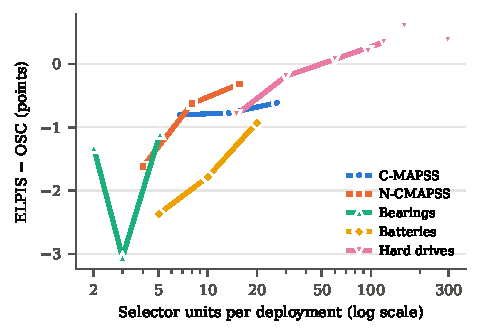
\includegraphics[width=\textwidth]{figures/learning_curve.pdf}
\caption{Gain of \RPT{} over \OSC{} (risk at 90\% matched coverage averaged over the six faults; points, negative is better) against the number of selector units per deployment. Benchmarks: all, half and a quarter of the selector units (exploratory, seeds 162--171, mean over 10 seeds). Hard drives: 15--120 subsampled units averaged over four drive-model sets, and all units for each set as unconnected markers (seeds 92--151). The benefit shrinks as selector data grow; on hard drives it is neutral at 30--60 units and a loss at 120 or more. The loss region is observed on hard drives only, where $D<0$; an optimism-inducing generator with $D>0$ gives the same curve there (Sec.~\ref{sec:hdd}), so the loss is caused by selector-set size.}
\label{fig:lc}
\end{figure}

\FloatBarrier
\FloatBarrier
\section{Discussion and limitations}
\begin{itemize}
\item \textbf{What \RPT{} teaches.} Large deviations on channel subsets, labelled by whether they actually make the predictor optimistic, show the selector which input deviations matter for the costly error; outlier labels, perturbation detectors and sensitivity features do not.
\item \textbf{Pessimistic errors.} One-sided selectors accept more pessimistic errors (2.5--4.8 points more than the best symmetric score). This is intended; a deployment that also penalises early predictions needs a two-sided cost.
\item \textbf{When it hurts, and what to deploy.} With plentiful selector data (hundreds of hard-drive units) perturbation training hurts. \AUTOD{} avoids this on our data but acts as a family-level switch and keeps less than half of the gain on bearings; a post hoc rule ``\RPT{} below 60 selector units, otherwise \OSC'' matches \AUTOD{} elsewhere and is 0.80 points better on bearings (not pre-registered).
\item \textbf{Multiplicity.} Ten confirmatory rounds spent $\alpha=0.04995$ of 0.05. Secondary families are tested at 0.05 within the family, and all results after round 10 (\EJG) are exploratory. Protocols were fixed in version-controlled files before each run.
\item \textbf{Scope.} The faults are injected apart from the battery jumps; a dedicated fault-robust RUL model was compared only in simplified form; ensembles have three members; and no finite-sample risk guarantee is available on the benchmark families. Appendix~\ref{app:discussion} discusses each point in full.
\end{itemize}

\FloatBarrier
\section{Conclusion}
Training a one-sided RUL selector on large random perturbations of channel subsets, each labelled by whether the fixed predictor becomes optimistic on it, gives a consistently better selector on four benchmark families, confirmed and replicated on fresh seeds and on rotated test units. On the windows a fault actually changes, the fault-induced excess falls where faults make the predictor optimistic. Perturbation training is a regulariser for scarce selector data: on real hard drives, with plentiful selector data, it hurts, whether or not the perturbations induce optimistic errors. The calibration-only gate (\AUTOD) was confirmed in four rounds: it was non-inferior on unseen drive models, and on 30 fresh seeds it was better than the selector without perturbations on all four benchmark families at the seed level and identical to it on hard drives. On bearings it keeps less than half of the gain of plain perturbation training. Plug-in thresholds keep the realised risk stable as fault prevalence rises but miss stated targets about half the time. Faults that mask degradation are beyond any input-based selector, and field-fault validation remains the main open step.


\FloatBarrier
\section{Data partitions}\label{app:splits}
\begin{table}[!htbp]
\caption{Units per partition for one seed (72; other seeds re-shuffle the same pools). C-MAPSS uses the official training engines only (50/10/15/10/15\%); the other families keep their official or condition-based evaluation units and split the remaining units into fit, validation, selector and calibration sets.}
\label{tab:splits}
\centering\footnotesize
\setlength{\tabcolsep}{3.5pt}
\resizebox{\textwidth}{!}{\begin{tabular}{lrrrrrr}
\toprule
Family (fold) & Channels & Fit & Valid. & Selector & Calib. & Eval.\\
\midrule
C-MAPSS FD001 / FD003 & 14 & 50 & 10 & 15 & 10 & 15\\
C-MAPSS FD002 & 14 & 130 & 26 & 39 & 26 & 39\\
C-MAPSS FD004 & 14 & 124 & 25 & 37 & 25 & 38\\
N-CMAPSS & 19 & 30 & 9 & 12 & 9 & 39\\
Bearings (per left-out condition) & 34 & 12--15 & 4 & 5--6 & 4 & 3--7\\
Batteries & 7 & 34 & 8 & 17 & 25 & 40\\
Hard drives & 17 & 739 & 222 & 296 & 222 & 612\\
Hard drives, unseen models & 17 & 399 & 120 & 160 & 120 & 361\\
\bottomrule
\end{tabular}}
\end{table}

\begin{table}[!htbp]
\caption{Descriptive differences on the round-7 and round-8 seeds (risk at 90\% matched coverage, six faults; points; negative favours the first method). Round 7: mean over 20 pairs, fifth column the fourth (unseen) drive-model set. Round 8: mean over 30 seeds, rotated N-CMAPSS and battery units, fifth column the original drive models. ``Signed-error regr.\ + pert.'' is signed-error regression trained on the same error-labelled perturbed windows as \RPT.}
\label{tab:r78}
\centering\footnotesize
\setlength{\tabcolsep}{3pt}
\resizebox{\textwidth}{!}{\begin{tabular}{lrrrrr}
\toprule
 & C-MAPSS & N-CMAPSS & Bearings & Batteries & Drives\\
\midrule
\multicolumn{6}{l}{\emph{Round 7 (seeds 152--161)}}\\
\RPT{} $-$ \OSC & $-0.64$ & $-0.50$ & $-0.81$ & $-0.51$ & $-0.11$\\
\AUTO{} $-$ \OSC & $-0.36$ & $-0.47$ & $-0.59$ & $-0.51$ & $-0.06$\\
\AUTOD{} $-$ \OSC & $-0.64$ & $-0.50$ & $-0.24$ & $-0.51$ & $+0.04$\\
\AUTOD{} $-$ Gaussian w/ bias~\cite{nix1994estimating} & $-0.97$ & $-0.27$ & $-0.28$ & $-0.30$ & $+0.05$\\
\AUTOD{} $-$ signed-error regr.~\cite{yoo2019learning} & $-1.50$ & $-0.37$ & $-0.01$ & $-0.30$ & $-0.25$\\
\AUTOD{} $-$ signed-error regr.\ + pert. & $-0.55$ & $+0.15$ & $+0.96$ & $+0.29$ & $-0.35$\\
\midrule
\multicolumn{6}{l}{\emph{Round 8 (seeds 162--191)}}\\
\RPT{} $-$ \OSC & $-0.64$ & $-0.29$ & $-1.43$ & $-1.04$ & $+0.41$\\
\AUTO{} $-$ \OSC & $-0.46$ & $-0.22$ & $-0.90$ & $-1.03$ & $+0.03$\\
\AUTOD{} $-$ \OSC & $-0.64$ & $-0.29$ & $-0.62$ & $-1.04$ & $0.00$\\
\AUTOD{} $-$ Gaussian w/ bias~\cite{nix1994estimating} & $-1.08$ & $-0.16$ & $-0.81$ & $-1.00$ & $+0.12$\\
\AUTOD{} $-$ signed-error regr.~\cite{yoo2019learning} & $-1.53$ & $-0.14$ & $-0.73$ & $-0.97$ & $+0.12$\\
\AUTOD{} $-$ signed-error regr.\ + pert. & $-0.48$ & $+0.07$ & $+1.01$ & $+0.08$ & $-0.44$\\
\midrule
\AUTOD{} switches to \RPT{} (round 8) & 100\% & 100\% & 42\% & 100\% & 0\%\\
\bottomrule
\end{tabular}}
\end{table}

\FloatBarrier
\section{Development of the switching rule (rounds 4--6)}\label{app:switch}
\paragraph{Round 4.} \AUTO{} chose \RPT{} in 50/80 C-MAPSS, 15/20 N-CMAPSS, 88/120 bearing, 18/20 battery and 4/20 hard-drive deployments of round 4. It gives up 0.28 points against \RPT{} on C-MAPSS, where its choice is noisy, and at most 0.07 on the other benchmark families, and it is what avoids the harm on hard drives ($-0.28$ against \RPT). Against the directional estimators it was better on C-MAPSS and bearings, not significantly different on N-CMAPSS and batteries, and slightly worse on hard drives ($+0.13$ and $+0.16$; $p_{\text{Holm}}=0.016$ and $0.0032$, the latter just above $\alpha_4$).
{\sloppy\begin{itemize}
\item \emph{\AUTO{} avoids the harm on the original drive models.} Its calibration check selects \OSC{} in 16 of 20 hard-drive deployments, and its risk equals that of \OSC{} ($+0.03$, n.s.). \OSC's own risk differs by 0.34 points between seed sets (15.44\% on seeds 42--51, 15.78\% on 92--101), as much as the harm of plain \RPT, so all comparisons are paired within a seed set. On the four benchmark families it keeps most of the gain of \RPT{} (Table~\ref{tab:confirm}).
\item \emph{An untouched test on unseen drive models.} Because hard-drive seeds 42--51 helped design \AUTO, we pre-registered a further test on drives of the next four most frequent failing models in the same archives (never loaded before), with fresh seeds 102--111 and no change to any method. Plain \RPT{} is again worse than \OSC{} ($+0.62$ points, 0 of 20 pairs), so the negative result replicates. \AUTO{} keeps \OSC{} in 14 of 20 deployments. Its pre-specified criterion (no significant loss against \OSC, mean difference at most $+0.3$) is formally met, but this is absence of evidence rather than evidence of no harm: it is worse by $+0.16$ points, in all 6 pairs where it chose \RPT{} and in none of the others ($p_{\text{Holm}}=0.055$), and significantly worse than the Gaussian with learned bias ($+0.27$, $p_{\text{Holm}}=0.017$). Its harm is smaller than that of plain \RPT{} ($-0.46$ points, 14 of 20 pairs, $p=0.001$), but every time it chose \RPT{} here, the choice was wrong. A seed-level bootstrap gives a 90\% interval of $[+0.04,+0.30]$ points: \AUTO{} is non-inferior to \OSC{} only at the pre-stated 0.3-point margin, and only just, while its 95\% interval $[+0.02,+0.32]$ excludes zero (on the original drive models, round 4: $[-0.01,+0.09]$). The calibration check therefore reduces but does not remove the risk of perturbation training on data where it does not help.
\item \emph{A stricter switch trades the benefit for safety (round 6).} On development data including the unseen drive models, a switching margin (choose \RPT{} only if its calibration risk is lower by more than one point) was the only candidate rule with no loss above 0.05 points on any family; requiring wins on all three seen shifts or a bootstrap probability of 0.8--0.9 was not safe. We confirmed it in a sixth pre-registered round on fresh seeds 142--151 and a third, untouched drive-model set (four further models, 679 drives). The margin rule never switched on the new drives and so equalled \OSC{} there, but it also switched rarely on the benchmark families (0--42\% of deployments) and gained only $-0.11$, $0.00$, $-0.47$ and $-0.12$ points, none significant at $\alpha_6$: the round failed its criterion. On the same seeds, plain \RPT{} was again worse than \OSC{} on the new drives ($+0.20$) and better on the benchmark families ($-0.30$ to $-1.15$), and the original \AUTO{} lost $+0.06$ on the drives while keeping $-0.19$ to $-0.80$ elsewhere. We found no calibration-risk rule that keeps the benefit and removes the harm, which led to the diagnostic switch below.
\end{itemize}}

\FloatBarrier
\section{Implementation details}\label{app:impl}
\paragraph{Predictors.} Each ensemble has three members trained from different seeds. GRU: two layers, 64 hidden units, dropout 0.1, linear head on the last state. TCN: a $1\times1$ input convolution to 64 channels followed by at least four residual causal blocks (kernel 3, dilations $1,2,4,8,\dots$, GELU, dropout 0.1), linear head on the last step. Loss: unit-weighted mean squared error on the capped target divided by the cap; AdamW (learning rate $10^{-3}$, weight decay $10^{-4}$), batch 128, at most 40 epochs with early stopping (patience 8) on the validation units. Windows and strides: C-MAPSS 30/5 (RUL cap 125), N-CMAPSS 10/1, bearings 30/5, batteries 30/10, hard drives 30/2. Inputs are $z$-scored on the fit units per operating regime (C-MAPSS, N-CMAPSS) or per drive model (hard drives); bearing and battery channels are first referenced to each unit's mean over its first ten records. Missing values are set to zero and flagged by indicator channels.
\paragraph{Selector features and classifier.} $\phi(x)$ contains the ensemble mean and standard deviation (divided by the cap on C-MAPSS), the elapsed time (cycle divided by the cap on C-MAPSS, $\log(1+t)$ elsewhere), and for every channel the window mean, the window standard deviation, the last-minus-first difference and the share of missing records. The classifier is scikit-learn's histogram gradient boosting with at most 7 leaves, at least 25 samples per leaf, $L_2$ penalty 2, 100 iterations and no early stopping, with unit-normalised sample weights.
\paragraph{Perturbation generator.} For each clean selector window and each of the $K=2$ copies, $k\sim\mathcal U\{1,\dots,\lfloor n/2\rceil\}$ channels are drawn without replacement. Each receives $A\,\varphi(t)$ with $\varphi(t)=\sum_{m=0}^{2}a_m\cos(\pi m t+b_m)$, $a_m\sim\mathcal N(0,1)$, $b_m\sim\mathcal U[0,2\pi)$, $t\in[0,1]$ over the window, normalised to $\max_t|\varphi(t)|=1$, and $\log A\sim\mathcal U[\log1,\log8]$ in normalised units; with probability 0.5 the perturbation is zero before a uniformly drawn onset. The diagnostic $D$ uses the same generator on the clean calibration windows with two further seeds.
\paragraph{Thresholds.} Matched coverage sets each score's threshold on the evaluated windows so that every selector accepts the same share; ties are broken by a fixed random key. Frozen thresholds (Sec.~\ref{sec:frozen}) are fitted on the clean calibration units.

\FloatBarrier
\section{Per-fault results}

\begin{table}[!htbp]
\caption{Round 2 (seeds 72--81): \RPT{} minus \OSC{} per fault (points).}
\label{tab:fault}
\centering\footnotesize
\begin{adjustbox}{max width=\textwidth}\begin{tabular}{lrrrr}
\toprule
Fault & C-MAPSS & N-CMAPSS & Bearings & Batteries\\
\midrule
Stuck-at & $-1.00$ & $-0.46$ & $-1.03$ & $-0.87$\\
Bias & $-0.95$ & $-0.42$ & $-1.38$ & $-3.17$\\
Noise & $-0.63$ & $-0.48$ & $-0.89$ & $-0.37$\\
Intermittent & $-0.06$ & $-0.30$ & $-1.01$ & $-0.14$\\
Spike & $-0.52$ & $-0.45$ & $-1.01$ & $-0.21$\\
Gain & $-0.13$ & $-0.30$ & $-1.03$ & $-0.63$\\
\bottomrule
\end{tabular}\end{adjustbox}
\end{table}

\FloatBarrier
\section{Proof of Proposition~\ref{prop:transfer}}\label{app:proof}
Write $\eta=\eta_Q$ and let $t$ and $\hat t$ be the coverage-$c$ thresholds of $\eta$ and $\hat\eta$ under $Q$, so that $g_\eta=\mathbf 1\{\eta\le t\}$ and $g_{\hat\eta}=\mathbf 1\{\hat\eta\le\hat t\}$ both accept mass exactly $c$. Let $A=\{g_{\hat\eta}=1,g_\eta=0\}$ and $B=\{g_{\hat\eta}=0,g_\eta=1\}$; since both selectors accept the same mass, $Q(A)=Q(B)$. Then
\begin{align*}
\Delta &:= c\,[R_Q(g_{\hat\eta})-R_Q(g_\eta)] = \mathbb E_Q[(g_{\hat\eta}-g_\eta)\eta]\\
&= \mathbb E_Q[(\eta-t)\mathbf 1_A]+\mathbb E_Q[(t-\eta)\mathbf 1_B]\\
&= \mathbb E_Q[(\eta-\hat\eta)\mathbf 1_A]+\mathbb E_Q[(\hat\eta-\eta)\mathbf 1_B]\\
&\quad+\mathbb E_Q[(\hat\eta-\hat t)\mathbf 1_A]-\mathbb E_Q[(\hat\eta-\hat t)\mathbf 1_B],
\end{align*}
where the terms in $t$ and $\hat t$ cancel because $Q(A)=Q(B)$. On $A$, $\hat\eta\le\hat t$; on $B$, $\hat\eta>\hat t$, so the last two terms are non-positive, and $\Delta\le\mathbb E_Q|\hat\eta-\eta|$. Under (A) and (B), $\mathbb E_Q|\hat\eta-\eta|=\mathbb E_P[w\,|\hat\eta-\eta|]\le\|w\|_{L_2(P)}\|\hat\eta-\eta\|_{L_2(P)}$ by Cauchy--Schwarz, and $\|w\|^2_{L_2(P)}=1+\chi^2(Q\|P)$. \qed


\FloatBarrier
\section{Detailed results}\label{app:detail}
Table~\ref{tab:claims} gives the evidential status of every claim.
\begin{table}[!htbp]
\caption{Status of the main claims. Confirmatory: pre-registered and tested once on never-used seeds within the $\alpha$-spending budget. Pre-registered secondary: fixed before the run, tested at 0.05 outside the budget; ``used seeds'' marks such analyses run on seeds already used for confirmation. Exploratory or post hoc: run on seeds already used, or defined after seeing results.}
\label{tab:claims}
\centering\footnotesize
\setlength{\tabcolsep}{3pt}
\begin{adjustbox}{max width=\textwidth}\begin{tabular}{@{}>{\raggedright\arraybackslash}p{0.60\textwidth}>{\raggedright\arraybackslash}p{0.36\textwidth}@{}}
\toprule
Claim & Status\\
\midrule
\RPT{} beats \OSC{} under six unseen faults on four benchmark families (rounds 2, 3) & confirmatory\\
\AUTOD{} beats \OSC{} on all four benchmark families at the seed level; equal on hard drives (round 8) & confirmatory\\
Fault-induced excess falls on affected windows (\AUTO: C-MAPSS, batteries, round 5; \AUTOD: C-MAPSS, N-CMAPSS, batteries, round 9) & confirmatory\\
\RPT{} beats sixteen external baselines & pre-registered secondary\\
\RPT{} hurts on real hard drives; \AUTO{} worse than \OSC{} on unseen drive models (95\% CI excludes 0) & pre-registered secondary\\
Labels, not perturbations, drive the gain (outlier exposure, volume, class balance) & pre-reg., used seeds\\
Gain grows as selector units shrink; harm on hard drives caused by selector-set size, not by $D$ (Fig.~\ref{fig:lc}, optimism-inducing generator) & exploratory\\
Sensitivity features do not replace perturbed copies & exploratory\\
\AUTOD{} beats \OSC{} also on the JEPA-pretrained predictor \EJ{} (round 10) & confirmatory\\
Lower risk at every coverage; expected cost & post hoc\\
Natural battery jumps & exploratory, replicated (pre-reg. secondary, round 9)\\
$D$ as a family-level gate (decision accuracy, robust and conservative predictors) & exploratory\\
\bottomrule
\end{tabular}\end{adjustbox}
\end{table}
\FloatBarrier
\subsection{Uncertainty and headroom}
\paragraph{Uncertainty from seeds and units.} The two backbones of a seed share a unit split, so the 20 pairs come from 10 independent splits. A hierarchical bootstrap over seeds (both backbones together) and, within each run, over test units (4\,000 replicates, thresholds fixed) gives 95\% intervals that exclude zero on every benchmark family, for \RPT{} $-$ \OSC{} in round 2 ($[-0.74,-0.37]$, $[-0.77,-0.10]$, $[-1.63,-0.48]$, $[-1.18,-0.63]$) and for \AUTO{} $-$ \OSC{} in round 4 ($[-0.68,-0.31]$, $[-0.55,-0.06]$, $[-1.71,-0.33]$, $[-1.01,-0.37]$; hard drives $[-0.01,+0.09]$). On N-CMAPSS the round-4 interval excludes zero although the Wilcoxon test missed $\alpha_4$. At the level of the 10 independent splits (GRU and TCN averaged), \RPT{} improves on \OSC{} in 10 of 10 seeds on every family in both round 2 and round 3, and \AUTO{} in 9--10 of 10 in round 4 (exact sign-flip $p=0.002$, the smallest attainable with 10 seeds, up to $0.014$). With Holm over the 12 tests of the round-2 family, even this minimum ($12\times0.002=0.023$) exceeds $\alpha_2$, so rounds 2--7 could not be confirmed at the seed level with 10 seeds (round 1, with Holm over 4, could: $4\times0.002<\alpha_1$); round 8 therefore used 30 seeds (Sec.~\ref{sec:hdd}); the confirmations rest on the pair-level tests, and the seed-level results show that they do not depend on a few seeds. Finally, the battery test cells are the same official cells for every seed. Rotating them in a five-fold split over all 124 cells (post hoc, seeds 122--131, 100 new ensembles) gives the same picture: \RPT{} $-$ \OSC{} is $-1.09$ points (20 of 20 pairs, 10 of 10 seeds, sign-flip $p=0.002$), negative in every fold ($-0.64$ to $-1.58$), and \RPT{} is better than both directional estimators ($-0.93$ and $-0.90$, 20 of 20 pairs). The same rotation over all 99 N-CMAPSS engines (seeds 132--141, 100 ensembles) gives a smaller but equally consistent gain: $-0.25$ points (20 of 20 pairs, 10 of 10 seeds; $-0.23$ to $-0.31$ in every fold), and $-0.11$ and $-0.09$ against the directional estimators (16 of 20 pairs). The gains therefore generalise to new units, not only to new training seeds.

\paragraph{Headroom (post hoc).} A hindsight oracle that rejects exactly the optimistic windows reaches a risk of $\max(0,r_{\text{all}}-0.1)/0.9$ at 90\% coverage, where $r_{\text{all}}$ is the rate when everything is accepted; both are computed per run and then averaged. On the round-8 runs (30 seeds; six faults; C-MAPSS, N-CMAPSS, bearings, batteries), accepting everything gives 11.2, 16.1, 26.4 and 7.4\%, and the oracle 2.4, 7.0, 18.7 and 1.1\%. \OSC{} closes 27, 87, 26 and 65\% of this gap and \AUTOD{} 34, 90, 34 and 81\%, i.e.\ 10, 25, 11 and 47\% of what \OSC{} leaves. The gains are small in points partly because little room is left on N-CMAPSS, and large room remains on C-MAPSS and bearings for any input-based selector.



\FloatBarrier
\subsection{Fault-specific gain}
A selector can improve under faults for two reasons: it handles faulty windows better (\emph{fault-specific} gain, measured by the fault-induced \emph{excess}, risk under a fault minus risk on the same windows without it), or it is simply a better selector (\emph{general} gain, visible on clean data). On whole test sets (Appendix Table~\ref{tab:excess}), \RPT{} almost removes the excess on C-MAPSS (0.69$\to$0.19 points, 20 of 20 pairs), also for the held-out ($-0.42$) and all-channel ($-0.55$) faults and the severe stress variants ($-0.86$). On the other families the whole-test excess barely changes ($-0.07$, $+0.01$, $-0.13$), most of the gain also appears on clean data ($-0.33$, $-1.07$, $-0.77$), and on bearings faults do not raise risk at all. Measured this way, \RPT{} would be a fault-specific improvement only on C-MAPSS and a better-regularised selector elsewhere; the next analysis shows that this measure is misleading.

\paragraph{Windows the fault actually changes (post hoc).} Whole-test excess understates the effect for two reasons (Table~\ref{tab:affected}). Each fault covers one interval and leaves about half of a faulty unit's windows unchanged, which dilutes it; and at fixed coverage, a selector that rejects more faulty windows must accept other, riskier windows instead, which raises its risk on the unchanged ones. On batteries, for example, the whole-test excess on these seeds is 0.97 for \OSC{} and 0.81 for \RPT, although on the affected windows it is 2.42 and 0.51: most of \RPT's whole-test excess comes from this re-allocation. Restricted to the affected windows, faults make the predictor more optimistic on three families (C-MAPSS, N-CMAPSS, batteries; by 2.6, 9.2 and 5.2 points) and \emph{less} optimistic on bearings and hard drives. On all three families where faults do harm the predictor, \RPT{} significantly lowers the fault-induced excess ($-1.22$, $-0.57$ and $-1.90$ points; 15--20 of 20 pairs), and \AUTO{} does so too ($-0.75$, $-0.40$, $-1.84$). On bearings and hard drives there is no fault-induced optimism to remove; on hard drives plain \RPT{} increases the excess, which \AUTO{} again avoids. The fault-specific gain therefore appears wherever faults make the predictor optimistic, not only on C-MAPSS; the general gain on clean data comes on top of it.

\paragraph{Confirmation on fresh seeds (round 5).} Because the affected-window analysis was post hoc, we pre-registered it as the primary endpoint of a fifth confirmatory round on 260 newly trained ensembles (seeds 112--121), with \AUTO{} unchanged. The excess falls significantly on C-MAPSS ($-0.89$ points, 19 of 20 pairs) and batteries ($-1.96$, 19 of 20) at $\alpha_5=0.0015625$, and by $-0.80$ on N-CMAPSS ($p_{\text{Holm}}=0.002$, short of $\alpha_5$); it is unchanged on bearings ($-0.18$) and hard drives ($+0.11$), and increases significantly on no family (Table~\ref{tab:confirm}). On whole test sets, \AUTO{} is again significantly better than \OSC{} on all four benchmark families ($-0.36$ to $-0.75$ points) and equal on hard drives ($+0.04$).

\paragraph{Naturally occurring glitches (exploratory, round-8 runs).} To test on faults we did not inject, we flagged physically implausible cycle-to-cycle jumps in the raw battery measurements, with thresholds fixed before any selector was scored: discharge or charge capacity more than 2\% from its 11-cycle running median, internal resistance more than 10\%, or a temperature more than 2\,\textdegree C. These glitches affect 0.4\% of cycles and 5.8\% of test windows, and they are harmful: on glitch windows the predictor is optimistic in 6.66\% of cases, against 3.02\% on non-glitch windows of the same cells within 50 cycles. At 90\% coverage, the optimistic rate among the accepted glitch windows is 0.61\% for \AUTOD{} and 2.14\% for \OSC{} ($-1.53$ points, 30 of 30 seeds, $p=2\times10^{-9}$), against 2.62--4.06\% for signed-error regression, the Gaussian with learned bias and ensemble spread. \AUTOD{} rejects 94\% of the optimistic glitch windows (\OSC{}: 79\%, ensemble spread: 55\%). The relative reduction on glitch windows (71\%) exceeds that on the other windows (41\%), so the gain is not only the general one. The seed-level $p$-value overstates the evidence across assets: pooling all runs per cell and resampling the 72 cells that have glitch windows gives a 95\% interval of $[-3.3,-0.1]$ points, and the difference comes from 15 cells (14 favour \AUTOD, one \OSC), because most cells have no accepted optimistic glitch window under either selector. A pre-registered replication on the round-9 seeds 192--221, with cell-level inference fixed in advance, confirms the result: the accepted-glitch-window optimistic rate is 0.71\% for \AUTOD{} and 2.51\% for \OSC{} (29 of 30 seeds), with a 95\% cell-bootstrap interval of $[-3.98,-0.15]$ points and 16 cells favouring \AUTOD{} against none favouring \OSC. Capacity can rebound genuinely after rest periods; using only the resistance and temperature channels (4.8\% of test windows) gives the same picture (accepted-window optimistic rate 0.66\% for \AUTOD{} and 2.20\% for \OSC, 30 of 30 seeds). A running-median rule may still flag some abrupt real degradation events, and the hard-drive data, which are cleaned by the provider and our preparation, contain almost no such glitches.

\paragraph{Confirmation for \AUTOD{} (round 9).} Round 5 confirmed the affected-window reduction for the earlier rule \AUTO. We therefore pre-registered the same primary endpoint for the recommended \AUTOD{} in a ninth round on 30 fresh seeds (192--221, 1\,260 ensembles, rotated N-CMAPSS and battery units), tested at the seed level. \AUTOD{} lowered the fault-induced excess on affected windows on C-MAPSS, N-CMAPSS and batteries by 1.10, 0.71 and 2.04 points (30 of 30 seeds each, $p_{\text{Holm}}=9\times10^{-9}$; $\alpha_9=0.0001$), left it unchanged on bearings ($-0.04$, 19 of 30, n.s.), where faults do not make the predictor optimistic, and equalled \OSC{} on hard drives, where it never switched. Pre-registered secondary results: whole-test risk under faults was again lower on all four benchmark families ($-0.28$ to $-1.04$ points, 29--30 of 30 seeds); the excess under the health-masking fault fell on C-MAPSS, N-CMAPSS and batteries ($-2.30$, $-0.26$, $-0.58$) but not on bearings ($+0.15$, n.s.); in the maintenance simulation with frozen thresholds failures were already near zero for every selector except on bearings, where \AUTOD{} lowered the failure rate from 9.40 to 8.65\%, at the cost of 0.2--0.6 more inspections per unit on the benchmark families.

\paragraph{Faults that mask degradation (round 5, secondary).} Our six faults rarely make the bearing and hard-drive predictors optimistic. We therefore designed, before round 5, a \emph{health-masking} fault: from late in life (60--75\% of elapsed life) to failure, three channels lose their slow trend and revert to the unit's early-life level, while their short-term fluctuation is kept. It makes the predictor optimistic on every family (on affected windows, 8.7$\to$37.5\% on C-MAPSS, 9.7$\to$59.4\% on batteries), but \AUTO{} reduces the resulting excess only on C-MAPSS ($-1.43$ points, 19 of 20 pairs; Holm over 5), not on the other families. A masked window is by construction an ordinary-looking healthy window, so the error event cannot be read from the input; this is exactly where the invariance assumption (A) of Prop.~\ref{prop:transfer} fails, and no input-based selector, including ours, can be expected to catch it. Redundant sensors or physical models are needed there. We also built, post hoc, a \emph{targeted} fault that is sure to move predictions: a $3\sigma$ bias on the three channels to which the predictor is most sensitive, in the direction that raises its RUL estimate (sensitivities from clean calibration windows; round-5 runs). It makes the predictor optimistic on every family (on affected windows, 17$\to$35\% on C-MAPSS, 22$\to$58\% on bearings, 18$\to$99\% on N-CMAPSS, 0.5$\to$96\% on batteries). \AUTO{} lowers the resulting excess on C-MAPSS ($-1.14$ points) and, for the first time, on bearings ($-1.03$; both $p_{\text{Holm}}=0.013$, Holm over 10), and by $-0.73$ on batteries (not significant after correction); on N-CMAPSS and batteries almost every affected window becomes optimistic, more than the 10\% a selector at 90\% coverage can reject, and on hard drives there is no reduction.




\FloatBarrier
\subsection{Baselines and fairness}\label{sec:fair}
These comparisons use \RPT. Because $D>0$ in all C-MAPSS and battery deployments and in 95--100\% of N-CMAPSS ones, \AUTOD{} coincides with \RPT{} on these families almost always and differs mainly on bearings and hard drives. Table~\ref{tab:sota} compares \RPT{} with sixteen external baselines and one variant of our method on the same fresh seeds and the same ensemble predictions, in a separately pre-registered family of 68 tests. Three further baselines were added post hoc on round-4 seeds 92--101: quantile regression of the signed error at level 0.9~\cite{koenker1978regression} (gradient-boosted, same features and data as \OSC), and PCA-based sensor validation by the residual (SPE/$Q$) statistic~\cite{jackson1979control} and Hotelling's $T^2$~\cite{macgregor1995statistical} (PCA on clean fit records, 95\% variance, window score the maximum over its records). \AUTO{} has lower risk than all three on all five families (by 0.35--2.44, 1.78--7.23 and 1.79--7.18 points; 18--20 of 20 pairs; Holm over 15), and so does \RPT{} (by 0.62--2.16, 1.85--7.29 and 1.86--7.24 points; 18--20 of 20 pairs). Finally, because no open implementation of a dedicated fault-robust RUL model was available, we built a simplified system after RobustUQ~\cite{wang2025robustuq} (separately pre-registered, round-8 seeds 162--171): suspicious channels are detected and reconstructed from the other channels, the fixed predictor is applied to the repaired window, and the score is the local 90\% quantile of the signed calibration residual among the nearest calibration windows in feature space (a $k$-nearest-neighbour stand-in for their metric learning; ridge reconstruction instead of their diffusion imputation). \AUTOD{} has lower risk than this system on C-MAPSS, N-CMAPSS, batteries and hard drives (by 1.72, 8.48, 2.84 and 4.33 points; 10 of 10 seeds; $p_{\text{Holm}}=0.0098$) but higher risk on bearings ($+2.35$, 1 of 10 seeds), where channel repair lowers the predictor's optimistic rate from 26.3 to 22.4\%, in line with the fault-detection-and-imputation result in Sec.~\ref{sec:fair}.
\begin{itemize}
\item \emph{Baselines.} Head-based baselines (Gaussian-NLL deep ensemble with three members, deep evidential regression with $\lambda=0.01$, SelectiveNet at target coverage 0.9, CQR with three $q=0.1$ members) are trained on clean fit units with early stopping on validation units. Last-layer Laplace (prior chosen by evidence), Mahalanobis and $k$-NN ($k{=}50$) distances on penultimate features are fitted on clean fit windows. The isolation forest uses selector features of clean selector windows. The analytic-redundancy residual is the maximum normalised residual of a per-channel ridge reconstruction. Test-time augmentation uses 10 draws of $\mathcal N(0,0.1^2)$ input noise. The Gaussian with learned bias~\cite{nix1994estimating} fits a gradient-boosted regressor $\hat\mu(x)$ of the signed error $E$ and a Poisson-loss regressor $\hat v(x)$ of the squared out-of-fold residual $E-\hat\mu$, and scores $\Phi\big((\hat\mu-\delta)/(\hat v+s^2_{\text{MC}})^{1/2}\big)$, where $s_{\text{MC}}$ is the MC-dropout spread. Signed-error regression scores by $\hat\mu(x)$ alone, a learned error predictor in the spirit of~\cite{yoo2019learning}. These and the other classifier- and regression-based baselines use the features, data and weights of \OSC; the fault detector is the same classifier trained to predict whether a training window was corrupted (dropout or drift) rather than whether the prediction is optimistic. Sparse white-noise training is round-1 perturbation training with a white-noise waveform. A distributional RUL model centred on its own prediction would score $P(Y<\hat y-\delta)=\Phi(-\delta/\hat\sigma)$, which ranks windows by $\hat\sigma$ alone; this is the Gaussian-NLL deep-ensemble row.
\item \emph{Result.} \RPT{} is significantly better in 67 of 68 comparisons and never significantly worse. Against the fourteen uncertainty, selective-prediction and anomaly baselines it lowers risk by 0.9--8.3 points, in 18--20 of 20 pairs. Against the directional estimators it is better by 0.25--1.79 points on every family. The only non-significant comparison is sparse white-noise training on C-MAPSS ($+0.05$), itself a variant of our approach.
\item \emph{Out-of-distribution and anomaly scores do not suffice.} Mahalanobis and nearest-neighbour feature distances, the isolation forest, the analytic-redundancy residual and a dedicated fault detector all perform at the level of ensemble spread. Detecting that an input is unusual is not the same as estimating whether the prediction is optimistic.
\item \emph{Clean data and pessimistic errors.} \RPT{} also has the lowest clean-data risk on every family. The one-sided selectors accept more pessimistic errors than the best symmetric or dispersion-based score, by 2.5--4.8 points; this is the intended trade-off of targeting optimistic errors.
\end{itemize}




Table~\ref{tab:fair} strengthens the baselines in four ways.
\begin{itemize}
\item \emph{Same perturbations for head-based baselines.} Retraining deep ensembles, evidential regression, CQR and SelectiveNet on clean plus perturbed windows does not close the gap: \RPT{} remains significantly better in all 16 comparisons. The perturbations help CQR on N-CMAPSS and batteries, but not the dispersion-based heads. The perturbed data alone does not explain the gain; a directional selector labelled by the predictor's own errors does.
\item \emph{A stronger error regression.} An absolute loss or a clipped target barely changes signed-error regression; its weakness on C-MAPSS (about 10.4\% risk) comes from the heavy-tailed signed error of a capped predictor. \RPT{} beats the strongest variant on every family.
\item \emph{Fault detection and imputation.} Repairing suspicious channels before prediction is the industrial default. With \OSC{} on top, it is significantly worse than \RPT{} on the turbofan families and batteries, but better on bearings (by 2.2 points; $p=0.05$ after Holm, not significant), where repair also lowers clean-data risk. Repair and \RPT{} are complementary on bearings: \RPT{} trained on repaired inputs has the lowest bearing risk of all systems (18.8\% against 22.0\% for \RPT{} alone; FDI + imputation + \RPT{} row of Table~\ref{tab:fair}), but it is worse on N-CMAPSS.
\item \emph{Larger ensembles.} With five members, ensemble spread improves by at most 0.3 points, and \RPT{} keeps its advantage in all 16 comparisons.
\end{itemize}


\FloatBarrier
\subsection{Stress tests, robust predictor and further checks}
\begin{table}[!htbp]
\caption{Four fault types designed after the method was frozen (clip, lag, quantisation, polarity inversion), seeds 72--81. Risk (\%) of \RPT{} and \RPT{} minus each baseline (points). \s: Holm over 20 tests, $\alpha=0.05$.}
\label{tab:heldout}
\centering\footnotesize
\begin{adjustbox}{max width=\textwidth}\begin{tabular}{lrrrr}
\toprule
 & C-MAPSS & N-CMAPSS & Bearings & Batteries\\
\midrule
Risk, \RPT & 9.46 & 8.84 & 22.19 & 3.81\\
\midrule
$-$ Ensemble spread~\cite{lakshminarayanan2017simple} & $-2.03$\s & $-7.15$\s & $-2.63$\s & $-1.68$\s\\
$-$ Gaussian w/ bias~\cite{nix1994estimating} & $-1.06$\s & $-0.23$\s & $-1.45$\s & $-0.74$\s\\
$-$ Signed-error regression~\cite{yoo2019learning} & $-1.71$\s & $-0.18$\s & $-1.01$\s & $-0.86$\s\\
$-$ \OSC & $-0.47$\s & $-0.33$\s & $-1.05$\s & $-1.00$\s\\
$-$ \Rone{} (round 1) & $-0.11$ & $-0.21$\s & $-0.78$\s & $-0.38$\s\\
\bottomrule
\end{tabular}\end{adjustbox}
\end{table}


\begin{itemize}
\item \emph{Held-out fault types (Table~\ref{tab:heldout}).} On four fault types that did not exist when the method was frozen, \RPT{} is significantly better than every external baseline on every family, and than the round-1 variant \Rone{} on three of four (tied on C-MAPSS).
\item \emph{Severity and channel count (Fig.~\ref{fig:sev}).} Across 13 scenarios (bias, noise, spike and gain at half and double severity; stuck and bias on 1 or 6 channels; noise on 6 channels), \RPT{} has lower risk than \OSC{} in 50 of 52 scenario--family cells (one tie, one $+0.04$), 41 of them significant after Holm over 260 tests. The gap to \OSC{} grows with noise severity on C-MAPSS, N-CMAPSS and batteries and stays at about 1 point on bearings; it grows with bias severity on C-MAPSS and bearings and stays roughly constant on N-CMAPSS and batteries. At the mildest noise level on batteries, the directional estimators are better than \RPT{} (by 0.43 points). On C-MAPSS, \RPT's risk barely changes from $1.5\sigma$ to $6\sigma$ bias, whereas every baseline degrades. On bearings, risk \emph{decreases} with fault severity for every method, so this family says little about fault robustness.
\item \emph{Physical faults on raw bearing signals.} Because bearing channels are derived features, we also injected five physical sensor faults into the \emph{raw} acceleration signals: sensitivity loss ($\times0.5$), amplifier saturation, a loosened mount (low-pass and attenuation), electrical noise and electromagnetic spikes. Features were then recomputed from the faulted signals. \RPT{} has 22.3\% risk, against 23.3 (\OSC), 23.4 (signed-error regression~\cite{yoo2019learning}), 23.7 (Gaussian with bias~\cite{nix1994estimating}) and 25.5\% (ensemble spread~\cite{lakshminarayanan2017simple}), significantly better than all four (Holm over 4; 17--20 of 20 pairs). It is lower than \OSC{} on every raw fault type, by 0.8--1.0 points. As on the injected bearing faults, the fault-induced excess is unchanged ($+0.13$, n.s.), so this is again a general improvement rather than a fault-specific one.
\end{itemize}



A natural alternative is to make the predictor itself robust by training it on the same perturbations (Table~\ref{tab:robust}). The result depends on the family. On C-MAPSS and bearings, the robust predictor is less accurate on clean data, and every robust system is significantly worse than the original predictor with \RPT, by 1.4--6.1 points. On N-CMAPSS and batteries, the robust predictor helps, and the best system combines it with \RPT; the differences are not significant, because systems with different predictors are compared: on batteries the per-pair difference between the two systems has a standard deviation of 2.7 points (8 of 20 pairs favour the original predictor), against 0.6 points for \RPT{} $-$ \OSC{} on the same predictor. With either predictor, \RPT{} improves on \OSC{} on all four families ($-0.43$, $-0.24$, $-1.28$ and $-0.82$ points with the robust predictor). Robust selection is thus a consistent improvement, and robust prediction is a complementary option whose value depends on the data.


\begin{itemize}
\item \emph{Error threshold.} Relabelling and re-evaluating with $\delta'=0.5\delta$ and $1.5\delta$, \RPT{} remains significantly better than \OSC{} on every family at both thresholds (8 of 8 tests, Holm; differences $-0.17$ to $-1.36$ points), and better than the other directional estimators and ensemble spread in all 24 comparisons.
\item \emph{Pessimistic errors priced in.} One-sided selectors trade pessimistic for optimistic errors. Combining the two rates at 90\% coverage as $r\cdot\text{optimistic}+\text{pessimistic}$, \RPT{} has the lowest cost among all external baselines on all four families for every cost ratio $r\ge2$. At $r=1$, a symmetric classifier (C-MAPSS, batteries) or SelectiveNet (bearings) is cheaper, and \RPT{} remains best only on N-CMAPSS. \RPT{} is therefore the right choice when an optimistic error costs at least twice a pessimistic one, which is the premise of safety-driven maintenance.
\item \emph{Ablations}\label{sec:abl}\emph{.} Appendix~\ref{app:extra} (Table~\ref{tab:abl}) tests expectations H1--H4. An unperturbed copy does not help (H1); small amplitudes and dense small noise are worse, while larger amplitudes and two copies tend to be better (significant only for two copies on C-MAPSS, $-0.15$) (H2, H3); the waveform, the constant term and the onset do not matter (H4); and reconstruction features help only on C-MAPSS, so the final method omits them.
\item \emph{Classifier}\label{sec:clf}\emph{.} Gradient boosting is the strongest selector model: logistic regression~\cite{cox1958regression}, a random forest~\cite{breiman2001random} and an MLP~\cite{rumelhart1986learning} are worse by up to 2.5 points and never better, consistent with tree ensembles' strength on tabular data~\cite{grinsztajn2022tree}. Default HGB hyperparameters give the same risk, and perturbation training helps every classifier (Appendix~\ref{app:extra}, Table~\ref{tab:clf}).
\item \emph{A third backbone}\label{sec:backbone}\emph{.} With Patch-Transformer backbones trained for 20 seeds (72--91; 20 pairs per family, one backbone; post hoc, Holm over 12), \RPT{} is significantly better than \OSC{} on all four families ($-0.51$, $-0.49$, $-1.69$ and $-0.84$ points; 19--20 of 20 pairs) and than both directional estimators on C-MAPSS, bearings and batteries ($-0.65$ to $-1.59$); on N-CMAPSS the difference to the directional estimators is $-0.15$ ($p_{\text{Holm}}=0.07$). \AUTO{} is also significantly better than \OSC{} on all four families ($-0.40$ to $-1.34$). The transformer is not uniformly stronger: its clean RMSE is worse than that of GRU/TCN on C-MAPSS (20.0 vs.\ 15.9 cycles on round-4 seeds; 16.1 on round-2 seeds, Table~\ref{tab:robust}) and bearings, similar on N-CMAPSS and better on batteries (0.122 vs.\ 0.131--0.144 on round-4 seeds, 0.124 on round-2 seeds), so the gain holds across predictors of different quality rather than shrinking with a weaker or stronger one. \emph{A larger predictor} (exploratory, C-MAPSS, round-8 seeds 162--171): doubling the hidden size to 128, using three recurrent layers and training for up to 100 epochs barely changes the all-window RMSE (15.39 vs.\ 15.55 cycles), and the gain of \AUTOD{} over \OSC{} is unchanged ($-0.62$ vs.\ $-0.61$ points, 10 of 10 seeds), as are its margins over the Gaussian with learned bias and signed-error regression ($-1.09$ and $-1.42$). \emph{A JEPA-pretrained predictor, \EJ} (exploratory, round-8 seeds 162--171; C-MAPSS, batteries, bearings): in the spirit of joint-embedding predictive architectures~\cite{assran2023ijepa}, we pretrained the encoder to predict, from a corrupted window (\RPT{} perturbations or contiguous channel masks), the latent that an EMA target encoder assigns to a clean window three steps later, and then fine-tuned it with a gated branch of per-channel trend features and observation quality. The resulting predictor is more accurate on C-MAPSS and batteries (RMSE 14.38 vs.\ 15.55 cycles; 0.086 vs.\ 0.094), and with it \AUTOD{} lowers risk under faults further (by 0.82 and 0.49 points against \AUTOD{} on the default predictor), but on bearings, with 12--15 fit units per condition, it is more optimistic under faults and worse by 3.30 points. An ablation without the self-supervised stage attributes the C-MAPSS gain mainly to the gated architecture and the battery gain to the pretraining, while on bearings both parts hurt. On bearings the pretrained predictor is biased towards optimism even on clean data; freezing the pretrained encoder in the supervised stage and subtracting the mean residual on validation units reduce the loss to $+1.08$ points (not significant) while keeping gains of $-0.42$ points on C-MAPSS and batteries, and with the same end-of-life offset applied to both predictors the pretrained one matches the default one in optimistic risk on bearings with fewer pessimistic errors ($-3.4$ points) and a lower RMSE (development results on used seeds, not confirmed). The complementarity, however, was confirmed: in a final pre-registered round on 30 fresh seeds with \EJ{}, the pretrained predictor with frozen encoder and validation bias correction, \AUTOD{} beat \OSC{} on C-MAPSS, batteries and bearings by 0.81, 1.14 and 1.03 points (30, 30 and 29 of 30 seeds; $p_{\text{Holm}}=6\times10^{-9}$; $\alpha_{10}=0.00005$), with pessimistic rises of at most 0.49 points. On the same fresh seeds, the full system with \EJ{} (descriptive comparison, not part of the confirmatory family) had lower risk than the system with the default predictor on C-MAPSS and batteries ($-0.60$ and $-0.45$ points; 24 and 21 of 30 seeds) and a lower RMSE on all three families, while on bearings it traded more optimistic errors ($+1.99$, 15 of 30 seeds, $p=0.15$) for 5.9 points fewer pessimistic ones. A pooled ensemble of the default and the \EJ{} members (selected on development seeds 162--171 and then evaluated, under a protocol fixed beforehand, on seeds 222--251; exploratory) had lower risk than the default predictor on C-MAPSS and batteries in both error types (optimistic $-0.66$ and $-0.67$ points, 28 and 30 of 30 seeds; pessimistic $-0.72$ and $-0.85$), and on bearings matched it in optimistic risk on average ($+0.35$ points, 15 of 30 seeds, $p=0.61$), although it missed the pre-specified non-inferiority margin of 0.3 points (upper 90\% bound 1.21), with 3.5 points fewer pessimistic errors and a lower RMSE (0.258 vs.\ 0.275). \EJG{}, which chooses between the default and the pooled predictor per deployment by the calibration risk of the selector that \AUTOD{} picks for each (calibration units only; a rule found post hoc on seeds 162--171 and 222--251), was then tested on 30 further fresh seeds 252--281 under a protocol fixed beforehand (exploratory): against \AUTOD{} on the default predictor it lowered risk under faults on C-MAPSS and batteries ($-0.58$ and $-0.54$ points, 29 and 30 of 30 seeds, $p<10^{-4}$) and on bearings by $-0.54$ points (90\% bootstrap interval $[-0.97,-0.13]$, 18 of 30 seeds, Wilcoxon $p=0.13$), meeting the pre-specified non-inferiority criterion but not the superiority criterion; pessimistic errors fell by 0.43--0.58 points on all three families. A pre-registered bearing replication on 60 further fresh seeds 282--341 gave $-0.56$ points (90\% interval $[-0.97,-0.14]$; 28 of 60 seeds, Wilcoxon $p=0.11$): the non-inferiority criterion was met again, the superiority criterion again not. With every predictor variant, \AUTOD{} remains better than \OSC{} on the same predictor ($-0.52$ to $-1.14$ points, the last confirmed in round 10; $-0.65$ to $-1.08$ on the pooled ensemble of \EJG), so the selector training is complementary to a stronger, fault-aware predictor.
\end{itemize}


\FloatBarrier
\subsection{Deployment, maintenance and cost}
With thresholds frozen on clean calibration units, \RPT{} has lower risk than \OSC, both directional estimators and ensemble spread on all four families (8.17, 7.51, 19.46 and 1.39\%, against at best 9.39, 8.40, 21.38 and 1.42\%). On the turbofan and bearing families, part of this comes from rejecting more (coverage 1.2--2.1 points below \OSC); on batteries, coverage is 1.3 points higher. Because frozen thresholds yield different coverages, these risks are not directly comparable; the matched-coverage results and Fig.~\ref{fig:rc} are the fair comparison. Coverage misses the 90\% target on bearings and batteries for every score, because calibration and evaluation units differ; the method offers relative robustness, not a coverage guarantee.

\paragraph{Deployment analyses (post hoc; Appendix~\ref{app:deploy}).} With thresholds fixed on calibration units and test mixtures in which up to half of the windows are faulty, the realised risk of \AUTO{} does not drift with fault prevalence (C-MAPSS: 5.36 to 5.16\% as prevalence rises from 0 to 0.5), unlike ensemble spread (5.95 to 6.91\%), and at the same risk target \AUTO{} keeps 7.7, 8.9 and 31.7 points more coverage than \OSC{} on C-MAPSS, bearings and batteries. A plug-in threshold is, however, no guarantee: it exceeds a stated risk target in 41--60\% of deployments, already without faults. Compared with a conservative offset alone, abstention plus a small offset reaches the target with a much smaller loss of accuracy. In a simple maintenance simulation of round 5 (replace when the accepted prediction falls below the critical RUL, inspect every abstained window), failures are almost entirely prevented by inspections for every selector, and \AUTO{} does not lower the total cost: it is costlier than \OSC{} on C-MAPSS, where it inspects more, and not significantly different elsewhere. Lower optimistic risk at fixed coverage does not by itself translate into lower maintenance cost under such a policy.

\paragraph{Expected cost (post hoc, round-8 runs).} Counting both error types at the same 90\% coverage, with cost $r\cdot$optimistic $+$ pessimistic, \AUTOD{} is cheaper than \OSC{} on all four benchmark families already at $r=1$ ($-0.17$, $-0.28$, $-0.37$ and $-0.81$ points on C-MAPSS, N-CMAPSS, bearings and batteries; 23--30 of 30 seeds), by 0.57--1.85 points at $r=2$ and by 2.85--10.18 points at $r=10$: the rise in pessimistic errors is smaller than the fall in optimistic ones. At every fixed coverage from 50 to 95\%, \AUTOD{} has a lower risk under the six faults than \OSC{} on all four benchmark families (0.07--1.65 points; 24--30 of 30 seeds), so at the same abstention budget it accepts fewer optimistic errors, at the price of slightly more pessimistic ones (up to 0.47 points at 90\% coverage). This is an average statement without a per-coverage test, and it does not contradict the maintenance simulation above, which inspects every abstained window and therefore prevents nearly all failures for every selector, so that its cost is driven by inspections alone. As a secondary, optimistic view, we also charge 1 per abstained window and $R$ per accepted optimistic error, and let each selector operate at its own cost-minimising coverage on the grid $\{0.5,0.6,0.7,0.8,0.85,0.9,0.95,1\}$. The coverage is chosen per run on the test curve, identically for all selectors, so the costs are optimistic for every method. With each selector at its own cost-minimising coverage, \AUTOD{} lowers the expected cost relative to \OSC{} on all four benchmark families for every $R$ from 2 to 50: by 2.0--11.5\% at $R=2$, 5.9--28.2\% at $R=10$ and 8.0--37.8\% at $R=50$ (smallest on C-MAPSS or bearings, largest on batteries; 26--30 of 30 seeds, for every family and $R$). On hard drives it equals \OSC. On clean data the reduction persists on N-CMAPSS, bearings and batteries (2--39\%) but not on C-MAPSS for $R\ge10$ ($-0.5$ to $+3.1$\%, n.s.).




\FloatBarrier
\subsection{Hard drives}
\begin{itemize}
\item \emph{One-sided selection still wins.} Every one-sided or directional selector beats ensemble spread by about 6 points.
\item \emph{Plain \RPT{} does not transfer.} It is significantly worse than \OSC{} under faults ($+0.36$ points, 0 of 20 pairs improved). Here the injected faults make the weak SMART predictor \emph{less} optimistic (its optimistic rate at full coverage falls from 24.0\% to 22.5\%), so the situation \RPT{} targets does not arise.
\item \emph{Calibration-risk switching (rounds 4--6, Appendix~\ref{app:switch}).} Plain \RPT{} was again worse than \OSC{} on a second, untouched set of four drive models ($+0.62$ points, 0 of 20 pairs). Choosing between \OSC{} and \RPT{} by their calibration risk (\AUTO) removed the harm on the original drive models but not on the unseen ones ($+0.16$ points, every switch wrong), and a stricter margin on that risk removed the benefit as well (round 6, not confirmed). This motivated the diagnostic below.
\item \emph{Why perturbation training fails on hard drives (post hoc).} Two measurements explain it. First, a diagnostic $D$ computed on calibration data only, the increase in the predictor's optimistic rate when the clean calibration windows are perturbed by the \RPT{} generator, is positive in all C-MAPSS and battery deployments and in 95\% of the N-CMAPSS ones (mean $+7$ to $+19$ points), but negative in all 80 hard-drive deployments across the three drive-model sets ($-1.9$ to $-2.4$ points): on these data the perturbations do not produce the optimistic errors that \RPT{} learns from. Using \RPT{} only when $D>0$ would have kept the gain on C-MAPSS, N-CMAPSS and batteries ($-0.74$, $-0.32$, $-0.72$ points), about half of it on bearings ($-0.43$, where $D$ is near zero), and caused no loss on any drive set. Second, the harm depends on the amount of selector data. Subsampling the hard-drive selector units, \RPT{} is clearly better than \OSC{} with 15 units ($-0.58$ to $-1.02$ points, 19--20 of 20 pairs on every drive set), neutral with 30--60 and worse only with 120 or more; the benchmark families have 5--39 selector units. Subsampling the benchmark selector units to a half and a quarter (exploratory, round-8 seeds 162--171) moves the same curve to the left (Fig.~\ref{fig:lc}): the gain of \RPT{} grows as selector units become scarcer on C-MAPSS ($-0.61$, $-0.78$, $-0.80$ points with all, half and a quarter of the units), N-CMAPSS ($-0.32$, $-0.63$, $-1.62$) and batteries ($-0.93$, $-1.79$, $-2.37$; 10 of 10 seeds in every cell), and stays large on bearings ($-1.11$, $-3.05$, $-1.32$ with 5, 3 and 2 units). \RPT{} thus acts as a regulariser that helps when selector data are scarce. A direct test separates selector-set size from the sign of $D$ (exploratory, round-8 drive runs): giving every channel's perturbation the sign that raises the predicted RUL makes $D>0$ in all 60 hard-drive deployments ($+3.6$ points on average), yet this optimism-inducing \RPT{} is still worse than \OSC{} with all 296 selector units ($+0.42$ points, 0 of 30 seeds), neutral-to-worse with 60 ($+0.16$) and better with 15 ($-0.65$, 28 of 30), exactly like plain \RPT. The harm on hard drives is therefore caused by the amount of selector data, not by the sign of $D$; $D$ gates correctly there only because $D<0$ coincides with large selector sets, and a gate on selector-set size explains our data at least as well.
\item \emph{A diagnostic switch, confirmed (round 7).} We pre-registered \AUTOD{} (use \RPT{} only if $D>0$) for a seventh round on fresh seeds 152--161 and a fourth, untouched set of drive models (the next four most frequent failing models; 349 drives, 109 test drives). It was significantly better than \OSC{} on C-MAPSS and N-CMAPSS ($-0.64$ and $-0.50$ points, 20 of 20 pairs each; Holm over 5 at $\alpha_7=0.00039$), by $-0.51$ on batteries ($p_{\text{Holm}}=0.0015$) and $-0.24$ on bearings (n.s.), and equal to \OSC{} on the new drives ($+0.04$; 90\% interval $[-0.03,+0.11]$, non-inferior at the pre-stated 0.3-point margin). On C-MAPSS it keeps the full gain of \RPT{} ($-0.64$), where the calibration-risk switch \AUTO{} kept only $-0.36$. On these drives $D$ was close to zero ($-0.6$ points on average) and \AUTOD{} switched in 8 of 20 deployments without harm. We therefore recommend \AUTOD{} over \AUTO{} (all round-7 and round-8 comparisons: Appendix Table~\ref{tab:r78}).
\item \emph{A seed-level confirmation (round 8).} Ten seeds cannot reach $\alpha$ at the seed level (Sec.~\ref{sec:results}), so we pre-registered a final round for \AUTOD{} alone: 30 fresh seeds (162--191, 1\,260 ensembles including N-CMAPSS and hard drives), rotated test units on N-CMAPSS and batteries, the original drive models, and a tighter non-inferiority margin of 0.15 points, with the seed (GRU and TCN averaged) as the unit. \AUTOD{} was better than \OSC{} on every benchmark family: by $0.64$, $0.29$, $0.62$ and $1.04$ points (C-MAPSS, N-CMAPSS, bearings, batteries), in 30, 30, 27 and 30 of 30 seeds ($p_{\text{Holm}}\le2\times10^{-7}$; 95\% seed-bootstrap intervals $[-0.72,-0.56]$, $[-0.33,-0.24]$, $[-0.81,-0.45]$, $[-1.15,-0.95]$), and by 0.62--1.16 points at 70\% coverage. Pessimistic errors rose by 0.01--0.47 points. On hard drives $D$ was negative in every deployment, so \AUTOD{} equalled \OSC{} exactly, whereas plain \RPT{} was worse ($+0.41$ points, 0 of 30 seeds). On bearings, where $D$ is near zero and \AUTOD{} switched in 42\% of deployments, it kept $-0.62$ of the $-1.43$ points that plain \RPT{} gained. \AUTOD{} was better than \OSC{} in each of the 20 disjoint test-unit sets (five battery and five N-CMAPSS folds, six bearing conditions, four C-MAPSS subsets), so the gain does not hinge on particular test assets. As a per-deployment predictor of whether \RPT{} helps, $D$ was right in 80\% of round-8 deployments (85--100\% on C-MAPSS, N-CMAPSS, batteries and hard drives; 46\% on bearings, where $D$ is near zero), but it does not rank the size of the gain (Spearman $\rho=0.01$): it acts as a family-level gate, not a fine-grained predictor. Making the predictor itself robust by training it on the same perturbations (exploratory, seeds 72--81) lowers $D$ (C-MAPSS $+5.9$, N-CMAPSS $+8.1$, batteries $+10.9$ points) but does not flip its sign, and \RPT{} still helps there ($-0.27$ to $-0.89$ points, 10 of 10 seeds); shifting every prediction down by $\delta$ or $2\delta$, as a conservative deployment would, also leaves $D>0$ on C-MAPSS, N-CMAPSS and batteries, while on bearings \RPT{} still helps in the deployments with $D\le0$ ($-1.08$ and $-0.20$ points). We found no benchmark setting in which $D\le0$ coincides with harm; harm with $D\le0$ appears only with the large hard-drive selector sets, so a gate on both $D$ and selector-set size fits all our data, but we have not confirmed it. The hard-drive test is non-significant by construction, because \AUTOD{} never switched there; with Holm over the four benchmark families alone the conclusions are the same.
\end{itemize}


\FloatBarrier
\subsection{Novelty controls}\label{app:novelty}
\begin{table}[!htbp]
\caption{Novelty controls, seeds 72--81: \RPT{} minus each variant (points). Top: same perturbed windows, other labels or estimators (\s: Holm over 20). Middle: same extra data volume without informative perturbations (tiny: $A\in[0.01,0.05]$), \OSC{} reweighted to \RPT's positive rate (\s: Holm over 8 per control pair), and an oracle trained on the evaluation faults (descriptive). Bottom: faults on \emph{all} channels, outside the generator's range (\s: Holm over 16). Exploratory.}
\label{tab:novelty}
\centering\footnotesize
\begin{adjustbox}{max width=\textwidth}\begin{tabular}{lrrrr}
\toprule
 & C-MAPSS & N-CMAPSS & Bear. & Batt.\\
\midrule
\multicolumn{5}{l}{\emph{Same perturbations, six unseen faults}}\\
Outlier-exposure labels~\cite{hendrycks2019deep} & $-1.63$\s & $-5.18$\s & $-2.33$\s & $-2.00$\s\\
Perturbation detector~\cite{isermann2005model} & $-2.49$\s & $-7.33$\s & $-2.73$\s & $-2.35$\s\\
Symmetric classifier~\cite{corbiere2019addressing,kamath2020selective} + pert. & $-3.54$\s & $-4.52$\s & $-4.09$\s & $-1.17$\s\\
Signed-error regr.~\cite{yoo2019learning} + pert. & $-0.77$\s & $+0.03$ & $+0.26$ & $+0.40$\s\\
Gaussian w/ bias~\cite{nix1994estimating} + pert. & $-0.38$\s & $+0.02$ & $-0.19$ & $+0.36$\s\\
\midrule
\multicolumn{5}{l}{\emph{Volume-matched controls and oracle (final configuration)}}\\
Two unperturbed copies & $-0.62$\s & $-0.42$\s & $-1.12$\s & $-1.00$\s\\
Two copies, tiny perturbations & $-0.57$\s & $-0.42$\s & $-1.23$\s & $-1.01$\s\\
Class reweighting & $-0.53$\s & $-0.39$\s & $-1.08$\s & $-0.90$\s\\
Oracle: train on the six test faults & $-0.15$ & $-0.09$ & $-1.04$ & $-0.16$\\
\midrule
\multicolumn{5}{l}{\emph{All-channel faults (bias $1\sigma$, stuck, gain $1.25$, noise $1\sigma$)}}\\
Risk, \RPT{} (\%) & 9.67 & 12.12 & 22.32 & 3.79\\
$-$ \OSC & $-0.60$\s & $-0.32$\s & $-1.13$\s & $-0.83$\s\\
$-$ Gaussian w/ bias~\cite{nix1994estimating} & $-1.32$\s & $-0.22$\s & $-1.42$\s & $-0.56$\s\\
$-$ Signed-error regression~\cite{yoo2019learning} & $-1.77$\s & $-0.25$\s & $-1.03$\s & $-0.60$\s\\
$-$ Ensemble spread~\cite{lakshminarayanan2017simple} & $-1.98$\s & $-7.54$\s & $-2.89$\s & $-1.84$\s\\
\bottomrule
\end{tabular}\end{adjustbox}
\end{table}

Is \RPT{} simply data augmentation or outlier exposure~\cite{hendrycks2019deep}? Table~\ref{tab:novelty} tests this on the same perturbed windows.
\begin{itemize}
\item \emph{The labels are the method.} Labelling every perturbed window as ``reject'', as outlier exposure would, is worse than \RPT{} by 1.6--5.2 points on every family. A detector of perturbed windows is worse still, and close to ensemble spread. Perturbations help only when each window is labelled by whether the fixed predictor actually becomes optimistic on it.
\item \emph{Perturbation content, not data volume.} Adding the same amount of extra data as two unperturbed copies, or with tiny perturbations, leaves risk at the level of \OSC{} on every family, on faults and on clean data alike. \RPT{} is significantly better than both controls on all four families. The clean-data improvement of \RPT{} therefore also comes from what the perturbations teach (how the predictor behaves under large input deviations), not from extra data volume: the regularisation comes from the informative labels, not from more samples.
\item \emph{Not a sensitivity feature (post hoc, round-7 runs).} Giving \OSC{} the predictor's response to a $\pm4\sigma$ offset on each single channel ($2n+2$ extra features per window) without perturbed copies leaves its risk unchanged ($-0.11$ to $+0.20$ points), and \RPT{} is better than this selector by 0.53--0.74 points on all four benchmark families (15--20 of 20 pairs, $p_{\text{Holm}}\le0.034$). Adding the same features to \RPT{} changes nothing ($-0.07$ to $+0.14$). The perturbed copies therefore do not teach the local sensitivity of a clean window; they extend the selector's training data into the region of input space where faults move test windows, labelled by the predictor's actual errors there.
\item \emph{Not a class-balance effect.} The perturbed copies raise the share of optimistic labels (on batteries from 4.6\% to 10.8\%), but reweighting \OSC's classes to the same share, or balancing them fully, leaves its risk unchanged, and \RPT{} remains significantly better on every family.
\item \emph{No better than training on the test faults.} A selector trained on the six evaluation faults themselves is not better than \RPT{} on any family (it is worse by 0.09--1.04 points; descriptive, not tested), and adding those faults to \RPT's training data changes risk by at most 0.01 points on every family (not shown in the table). The random perturbations already convey what the evaluation faults would; the oracle is worse on bearings plausibly because six fault types, each with few selector units, regularise the selector less than the varied random perturbations do.
\item \emph{The target must be directional.} A symmetric $|E|>\delta$ classifier does not benefit from the same data.
\item \emph{Error-labelled perturbations transfer to other directional estimators.} Trained on the same perturbed windows, signed-error regression and the Gaussian with learned bias improve markedly and match \RPT{} on N-CMAPSS and bearings. On batteries they are slightly better (by 0.36--0.40 points); on C-MAPSS the classifier remains best. Against the recommended \AUTOD, perturbation-trained signed-error regression is also better on bearings (by about 1 point in rounds 7 and 8, Table~\ref{tab:r78}), because \AUTOD{} keeps \OSC{} in more than half of the bearing deployments, and worse on C-MAPSS and hard drives. The contribution is therefore the training scheme (error-labelled perturbations for a directional estimator) rather than a particular estimator. We keep the classifier because the pre-registered selection rule chose it: on development seeds, the directional regressors trained with perturbations were worse than \OSC{} on C-MAPSS (by 0.12--0.53 points) and so failed the safety condition.
\item \emph{Beyond the generator's range.} Faults that hit all channels lie outside the generator's parameter range, which perturbs at most half of the channels. On these faults \RPT{} remains significantly better than every baseline on every family.
\item \emph{Overlap does not explain the gain.} We trained classifiers to separate perturbed windows from truly faulty windows. Most faults are clearly separable from the perturbations in the selector's feature space (2-fold AUC $>0.8$ in 39 of 56 fault--family cells; the exception is bearings, whose 34 derived features overlap broadly, AUC 0.54--0.78 for most faults). We found no clear relation between this overlap and the gain over \OSC{} (Spearman $\rho=0.23$, $p=0.10$, cells not independent), which argues against the gain coming only from faults that resemble the perturbations.
\end{itemize}

\begin{table}[!htbp]
\caption{Confirmatory rounds 1--7 (the final rounds 8--10 are in Table~\ref{tab:confirm}). Risk is the optimistic-error rate (\%) at 90\% matched coverage, averaged over six unseen faults; differences in points with pairs improved out of 20 and Holm-adjusted $p$. Round 1: \Rone{} vs.\ \OSC, seeds 62--71, Holm over 4, $\alpha_1=0.025$. Round 2: \RPT{} vs.\ three comparators, seeds 72--81, Holm over 12, $\alpha_2=0.0125$. Round 3: unchanged \RPT{} replicated on seeds 82--91 (Holm over 12, $\alpha_3=0.00625$). Round 4: \AUTO{} on seeds 92--101 across five families including hard drives (Holm over 15, $\alpha_4=0.003125$; significant on C-MAPSS, bearings and batteries, not on N-CMAPSS). Round 5: fault-induced excess on affected windows, \AUTO{} vs.\ \OSC, seeds 112--121 (Holm over 5, $\alpha_5=0.0015625$; significant on C-MAPSS and batteries; hard drives: $+0.11$, 0 of 20 pairs improved, $p=0.18$). Round 6 (not confirmed): a margin switch, seeds 142--151 (Holm over 5, $\alpha_6=0.00078$). Round 7: \AUTOD{} vs.\ \OSC, seeds 152--161 (Holm over 5, $\alpha_7=0.00039$; significant on C-MAPSS and N-CMAPSS; unseen drive models non-inferior). ``Points'' are percentage points throughout.}
\label{tab:history}
\centering\footnotesize
\resizebox{\textwidth}{!}{\begin{tabular}{lrrrr}
\toprule
 & C-MAPSS & N-CMAPSS & Bearings & Batteries\\
\midrule
\multicolumn{5}{l}{\emph{Round 1 (seeds 62--71)}}\\
\Rone{} $-$ \OSC & $-0.52$ & $-0.14$ & $-0.55$ & $-0.32$\\
\quad pairs / $p$ & 20, 1e-5 & 17, 6e-4 & 17, 3e-4 & 18, 0.003\\
\midrule
\multicolumn{5}{l}{\emph{Round 2 (seeds 72--81)}}\\
Risk, \OSC & 9.52 & 10.21 & 23.04 & 4.29\\
Risk, \RPT & \textbf{8.97} & \textbf{9.81} & \textbf{21.98} & \textbf{3.39}\\
\RPT{} $-$ \OSC & $-0.55$ & $-0.40$ & $-1.06$ & $-0.90$\\
\quad pairs / $p$ & 19, 4e-5 & 18, 7e-5 & 19, 4e-5 & 19, 4e-5\\
\RPT{} $-$ Gaussian w/ bias~\cite{nix1994estimating} & $-1.15$ & $-0.25$ & $-1.48$ & $-0.54$\\
\quad pairs / $p$ & 20, 2e-5 & 17, 0.001 & 19, 8e-5 & 16, 0.004\\
\RPT{} $-$ signed-error regr.~\cite{yoo2019learning} & $-1.79$ & $-0.25$ & $-1.03$ & $-0.55$\\
\quad pairs / $p$ & 20, 2e-5 & 17, 3e-4 & 17, 5e-4 & 17, 0.004\\
Relative to \OSC & $-5.8\%$ & $-3.9\%$ & $-4.6\%$ & $-21\%$\\
Pessimistic change vs.\ \OSC & $+0.33$ & $+0.03$ & $+0.65$ & $+0.62$\\
Clean risk, \OSC{} $\to$ \RPT & 8.83$\to$8.78 & 6.77$\to$6.44 & 23.2$\to$22.2 & 2.84$\to$2.08\\
\midrule
\multicolumn{5}{l}{\emph{Round 3, replication (seeds 82--91), $\alpha_3=0.00625$}}\\
\RPT{} $-$ \OSC & $-0.70$ & $-0.34$ & $-1.56$ & $-0.73$\\
\quad pairs / $p$ & 20, 2e-5 & 20, 2e-5 & 19, 3e-5 & 19, 3e-5\\
\RPT{} $-$ Gaussian w/ bias~\cite{nix1994estimating} & $-1.24$ & $-0.27$ & $-1.73$ & $-0.41$\\
\quad pairs / $p$ & 20, 2e-5 & 16, 0.002 & 18, 6e-5 & 15, 0.1\\
\RPT{} $-$ signed-error regr.~\cite{yoo2019learning} & $-1.82$ & $-0.28$ & $-1.63$ & $-0.45$\\
\quad pairs / $p$ & 20, 2e-5 & 16, 0.002 & 18, 7e-5 & 15, 0.1\\
\midrule
\multicolumn{5}{l}{\emph{Round 4: \AUTO, seeds 92--101, $\alpha_4=0.003125$ (fifth family: Table~\ref{tab:hdd})}}\\
\AUTO{} $-$ \OSC & $-0.49$ & $-0.27$ & $-1.05$ & $-0.67$\\
\quad pairs / $p$ & 20, 3e-5 & 15, 0.005 & 17, 0.002 & 17, 0.002\\
\midrule
\multicolumn{5}{l}{\emph{Round 5: \AUTO, seeds 112--121, $\alpha_5=0.0015625$; excess on affected windows}}\\
$\Delta$excess, \AUTO{} $-$ \OSC & $-0.89$ & $-0.80$ & $-0.18$ & $-1.96$\\
\quad pairs / $p$ & 19, 2e-5 & 14, 0.002 & 13, 0.11 & 19, 5e-4\\
\midrule
\multicolumn{5}{l}{\emph{Round 6: switching margin 0.01, seeds 142--151, $\alpha_6=0.00078$ (not confirmed)}}\\
Margin rule $-$ \OSC & $-0.11$ & $0.00$ & $-0.47$ & $-0.12$\\
\quad pairs / $p$ & 9, 0.07 & 0, 1 & 14, 0.02 & 7, 0.28\\
\midrule
\multicolumn{5}{l}{\emph{Round 7: \AUTOD, seeds 152--161, $\alpha_7=0.00039$ (fifth family: unseen drive models, $+0.04$, n.s.)}}\\
\AUTOD{} $-$ \OSC & $-0.64$ & $-0.50$ & $-0.24$ & $-0.51$\\
\quad pairs / $p$ & 20, 1e-5 & 20, 1e-5 & 12, 0.16 & 17, 0.0015\\
\bottomrule
\end{tabular}}
\end{table}


\FloatBarrier
\section{Extended discussion}\label{app:discussion}
\begin{itemize}
\item \textbf{What \RPT{} teaches the selector.} Large deviations on subsets of channels, labelled by whether they actually make the predictor optimistic, teach the selector which input deviations matter for the costly error. Outlier-exposure labels and perturbation detectors fail, and explicit single-channel sensitivity features do not replace the perturbed copies, so the selector learns where large deviations make the predictor optimistic, not input novelty or local sensitivity. Amplitude matters, the waveform does not, and the gains extend to faults outside the generator's parameter range. Prop.~\ref{prop:transfer} is only a heuristic account of this.
\item \textbf{Pessimistic errors.} One-sided selectors accept more pessimistic errors than symmetric or dispersion-based scores (2.5--4.8 points more than the best such baseline on seeds 72--81). This is the intended trade-off; a deployment that also penalises early predictions would need a two-sided cost.
\item \textbf{When perturbation training hurts, and what to deploy.} On real hard-drive failures plain \RPT{} is worse than \OSC. A direct test (Sec.~\ref{sec:hdd}) shows that this is caused by the large selector sets, not by whether the perturbations induce optimistic errors: an optimism-inducing generator hurts just as much with 296 selector units and helps with 15. The pre-registered gate \AUTOD{} avoids the harm on hard drives and was confirmed in four rounds, but it acts as a family-level switch: it equals \RPT{} on C-MAPSS, N-CMAPSS and batteries, equals \OSC{} on hard drives, and on bearings, where $D$ is near zero, it keeps less than half of the gain of \RPT. Our practical recommendation is therefore to use \RPT{} when selector data are scarce (tens of units, as in all four benchmark families) and \OSC{} with hundreds of units; \AUTOD{} is a calibration-only safeguard that implements this choice correctly on our data, but a gate on selector-set size explains the evidence at least as well. Re-scoring the round-9 runs post hoc (seeds 192--221, which played no part in choosing the size threshold of about 60 units from the learning curves) with the rule ``use \RPT{} below 60 selector units, otherwise \OSC'' gives the same result as \AUTOD{} on C-MAPSS, N-CMAPSS, batteries and hard drives and is better on bearings by 0.80 points (28 of 30 seeds), recovering the full gain of \RPT{} there ($-1.37$ points against \OSC). This rule was not pre-registered, and the $\alpha$ budget does not allow a further confirmatory round.
\item \textbf{Multiplicity.} Development seeds were reused while the method was developed. The ten confirmatory rounds spent $\alpha=0.04995$ of a 0.05 budget; the last tests the recommended method alone at the seed level, so its conclusion does not rest on treating the two backbones of a seed as independent. Because the generator was selected on development seeds scored on the same six fault types, we re-ran the round-2 selection rule post hoc with each fault type left out, and with only \{stuck, bias, noise\} or only \{intermittent, spike, gain\}: in all eight cases it picks one of the three large-amplitude variants ($A\in[1,8]$, at most half of the channels; smooth, white or with reconstruction features), and \RPT{} is within 0.1 points of the selected candidate. The essential choice therefore does not depend on which faults were used for selection; the four held-out fault types (Table~\ref{tab:heldout}) test it on faults that played no part in it. Secondary pre-registered families (for example the 68 baseline tests) are tested at 0.05 within their family, outside the $\alpha$ budget, so their significance marks carry no family-wise guarantee across families. Protocols were fixed in version-controlled files before each run, not on a public registry. The analyses after confirmation were pre-registered but ran on seeds already used for confirmation. Ablations and the classifier study are exploratory.
\item \textbf{What the gain is.} Two parts. On the windows a fault changes, the fault-induced excess falls on the three families where faults make the predictor optimistic (C-MAPSS, N-CMAPSS, batteries; confirmed for \AUTO{} on C-MAPSS and batteries in round 5); on whole test sets this is visible only on C-MAPSS, because unchanged windows and the re-allocation of coverage hide it. Faults that mask degradation are not caught. Separately, much of the gain also appears on clean data, so \RPT{} is also a better-regularised selector. Bearings and hard drives do not stress-test fault robustness, since our faults make their predictors less, not more, optimistic. On batteries, directional regressors trained with the same error-labelled perturbations are slightly better than the classifier.
\item \textbf{Scope.} The faults are injected, apart from the natural battery glitches of Sec.~\ref{sec:excess}, although eight of them (held-out and all-channel) were designed only after the method was frozen. We compared with a dedicated fault-robust RUL model only in a simplified form after~\cite{wang2025robustuq} (Sec.~\ref{sec:sota}), and with a predictor trained on the same perturbations (Sec.~\ref{sec:robust}). Ensembles have three members. \OSC{} is the selector of an earlier study under review; Sec.~\ref{sec:method} describes it completely, so the results here do not depend on that paper. No finite-sample guarantee is available on the benchmark families. In a separate study, Learn-then-Test~\cite{angelopoulos2021ltt} with Hoeffding, Bernstein and betting~\cite{waudbysmith2024betting} bounds, treating units as exchangeable, certified no threshold with the labelled units available per deployment on the benchmark families (4--26 calibration units here, up to 71 when the four C-MAPSS subsets are pooled), even for the weakest target (risk no higher than accepting everything); a power calculation put the requirement at $10^2$--$10^3$ units. On hard drives, where each deployment has 222 calibration units, the betting bound does certify the weakest target in every deployment (95\% coverage, risk no higher than accepting everything; no violation on clean test units, failure probability $\epsilon=0.1$), a 15\% reduction in 4 of 40 deployments and a 30\% reduction in none; with 120 units (unseen drive models) it certifies nothing (Appendix~\ref{app:deploy}).
\end{itemize}


\FloatBarrier
\section{Additional results}\label{app:extra}
\begin{table}[!htbp]
\caption{Ablations, risk (\%) at 90\% matched coverage, six unseen faults. Top, seeds 72--81 (descriptive): variants on the path from \OSC{} to \RPT. Bottom, seeds 62--71: variants of \Rone{}, minus \Rone{} (points); \s: Holm over 44, exploratory.}
\label{tab:abl}
\centering\footnotesize
\resizebox{\textwidth}{!}{\begin{tabular}{lrrrr}
\toprule
 & C-MAPSS & N-CMAPSS & Bear. & Batt.\\
\midrule
\multicolumn{5}{l}{\emph{Seeds 72--81, risk (\%)}}\\
\OSC{} (no perturbation) & 9.52 & 10.21 & 23.04 & 4.29\\
+ \RPT, $K{=}1$, $\rho{=}0.2$, $A\in[0.5,4]$ & 9.24 & 9.94 & 22.85 & 3.53\\
\quad same, white-noise waveform & 9.25 & 9.95 & 22.79 & 3.72\\
+ \RPT, $K{=}2$, $\rho{=}0.5$, $A\in[1,8]$ (final) & 8.97 & 9.81 & 21.98 & 3.39\\
\quad same, white-noise waveform & 9.06 & 9.82 & 22.10 & 3.28\\
\quad same, + reconstruction features & 8.74 & 9.87 & 21.95 & 3.60\\
\midrule
\multicolumn{5}{l}{\emph{Seeds 62--71, variant minus \Rone{} (points)}}\\
Unperturbed copy (H1) & $+0.26$\s & $+0.28$\s & $+0.40$ & $+0.40$\s\\
Small amplitude, $A\in[0.25,1]$ (H2) & $+0.21$\s & $+0.07$ & $+0.47$ & $+0.27$\s\\
Large amplitude, $A\in[2,8]$ (H2) & $-0.15$ & $-0.05$ & $-0.38$ & $-0.04$\\
Dense noise, all channels~\cite{bishop1995training} (H3) & $+0.23$\s & $+0.07$ & $+0.12$ & $+0.34$\s\\
One channel, $k=1$ (H3) & $0.00$ & $+0.08$\s & $+0.37$ & $0.00$\\
No constant term, $a_0=0$ (H4) & $-0.05$ & $+0.01$ & $+0.09$ & $+0.02$\\
No onset (H4) & $-0.06$ & $-0.02$ & $+0.13$ & $+0.06$\\
White-noise waveform (H4) & $+0.03$ & $-0.01$ & $+0.21$ & $+0.11$\\
Two perturbed copies & $-0.15$\s & $-0.05$ & $+0.03$ & $-0.09$\\
Without dropout and drift & $-0.03$ & $+0.07$ & $-0.01$ & $-0.06$\\
Oracle: train on the 6 test faults & $-0.16$ & $-0.08$ & $+0.16$ & $+0.03$\\
\bottomrule
\end{tabular}}
\end{table}

Table~\ref{tab:abl} tests expectations H1--H4.
\begin{itemize}
\item \emph{(H1) Support, not data.} An unperturbed copy with the same weights is significantly worse than \Rone{} on three families.
\item \emph{(H2) Amplitude.} Small amplitudes are worse, larger ones better. Moving from the round-1 generator to the final one (larger amplitude, more channels, two copies) lowers risk on every family on fresh seeds.
\item \emph{(H3) Sparsity.} Dense small noise on all channels, the classic augmentation~\cite{bishop1995training}, is significantly worse on two families.
\item \emph{(H4) Waveform.} Removing the constant term or the onset, or replacing the smooth waveform by white noise, changes risk by at most 0.21 points, never significantly; on fresh seeds the two waveforms are within 0.19 points. In particular, the gain on bias faults does not come from the generator's constant term.
\item \emph{Other components.} Reconstruction features help on C-MAPSS but not elsewhere, so the final method omits them. \RPT{} can also replace the hand-designed dropout and drift shifts.
\item \emph{Training on the test faults.} A selector trained on the six evaluation faults themselves (with \Rone's features) improves on \Rone{} by at most 0.16 points; since the final \RPT{} improves on \Rone{} by more, this is not an upper bound for the final configuration.
\end{itemize}




\begin{table}[!htbp]
\caption{Classifier study, seeds 62--71 (points; exploratory, \s: Holm over 32). Top: classifier minus histogram gradient boosting (HGB~\cite{ke2017lightgbm,pedregosa2011scikit}) with the \OSC{} features, data and weights. Bottom: gain of perturbation training (round-1 generator) per classifier.}
\label{tab:clf}
\centering\footnotesize
\begin{adjustbox}{max width=\textwidth}\begin{tabular}{lrrrr}
\toprule
 & C-MAPSS & N-CMAPSS & Bear. & Batt.\\
\midrule
Logistic regression~\cite{cox1958regression} $-$ HGB & $+1.10$\s & $+2.45$\s & $+0.87$\s & $+0.15$\\
Random forest~\cite{breiman2001random} $-$ HGB & $+0.70$\s & $+1.94$\s & $+0.44$ & $+0.37$\\
MLP (64, 64)~\cite{rumelhart1986learning} $-$ HGB & $+1.65$\s & $+2.54$\s & $+1.23$\s & $+0.81$\s\\
HGB defaults $-$ HGB & $+0.06$ & $0.00$ & $+0.01$ & $+0.19$\\
\midrule
Gain, logistic regression~\cite{cox1958regression} & $-0.40$\s & $-1.45$\s & $-1.33$\s & $-0.36$\s\\
Gain, random forest~\cite{breiman2001random} & $-0.72$\s & $-0.92$\s & $-0.16$ & $-0.17$\s\\
Gain, MLP~\cite{rumelhart1986learning} & $-0.73$\s & $-1.29$\s & $-0.43$ & $-0.60$\s\\
Gain, HGB defaults & $-0.62$\s & $-0.17$\s & $-0.30$ & $-0.53$\s\\
\bottomrule
\end{tabular}\end{adjustbox}
\end{table}

\paragraph{Classifier study.}
Gradient boosting is the strongest selector model (Table~\ref{tab:clf}). Logistic regression, a random forest and an MLP are worse by up to 2.5 points and never better, consistent with tree ensembles' strength on medium-sized tabular data~\cite{grinsztajn2022tree}. HGB's default hyperparameters give the same risk as the pre-specified ones. Perturbation training helps every classifier on every family, significantly in 13 of 16 cases, so the gain is not specific to boosting.



\begin{table}[!htbp]
\caption{How much of the gain is fault-specific? Round 2 (seeds 72--81): risk (\%) under the six faults, on clean data, and the fault-induced excess (difference). Last row: excess of \RPT{} minus excess of \OSC, per pair (pairs improved; Wilcoxon $p$).}
\label{tab:excess}
\centering\footnotesize
\begin{adjustbox}{max width=\textwidth}\begin{tabular}{lrrrr}
\toprule
 & C-MAPSS & N-CMAPSS & Bear. & Batt.\\
\midrule
\OSC, faults & 9.52 & 10.21 & 23.04 & 4.29\\
\OSC, clean & 8.83 & 6.77 & 23.22 & 2.84\\
\OSC, excess & 0.69 & 3.44 & $-0.18$ & 1.44\\
\RPT, faults & 8.97 & 9.81 & 21.98 & 3.39\\
\RPT, clean & 8.78 & 6.44 & 22.16 & 2.08\\
\RPT, excess & 0.19 & 3.37 & $-0.17$ & 1.31\\
Gaussian w/ bias~\cite{nix1994estimating}, excess & 0.83 & 3.43 & $-0.14$ & 1.66\\
Ensemble spread~\cite{lakshminarayanan2017simple}, excess & 1.07 & 4.39 & 0.13 & 2.22\\
\midrule
$\Delta$excess, \RPT{} $-$ \OSC & $-0.50$ & $-0.07$ & $+0.01$ & $-0.13$\\
\quad pairs improved / $p$ & 20, $<$1e-4 & 10, 0.8 & 12, 0.6 & 13, 0.3\\
\bottomrule
\end{tabular}\end{adjustbox}
\end{table}

% moved from the main text
\begin{table}[!htbp]
\caption{Fairness checks, seeds 72--81: \RPT{} minus each strengthened baseline (points; \s: Holm within each block). Top: head-based baselines retrained on clean plus perturbed windows (same generator, true labels; Holm over 16). Second block: the strongest signed-error-regression variant per family (absolute loss or clipped target, chosen on these seeds in the baseline's favour; Holm over 4). Third block: the industrial default of detecting faulty channels by analytic redundancy, replacing them by their reconstruction and predicting from the repaired input; each system ranks its own predictions (Holm over 8 for the first two rows; the last row is descriptive). Bottom: all methods on 5-member ensembles (Holm over 16).}
\label{tab:fair}
\centering\footnotesize
\begin{adjustbox}{max width=\textwidth}\begin{tabular}{lrrrr}
\toprule
 & C-MAPSS & N-CMAPSS & Bear. & Batt.\\
\midrule
\multicolumn{5}{l}{\emph{Head baselines trained with perturbations}}\\
Deep ensemble, Gaussian NLL~\cite{lakshminarayanan2017simple} & $-2.04$\s & $-7.22$\s & $-4.03$\s & $-1.84$\s\\
Deep evidential regression~\cite{amini2020deep} & $-2.36$\s & $-7.32$\s & $-4.08$\s & $-1.90$\s\\
CQR lower bound~\cite{romano2019cqr} & $-1.09$\s & $-3.74$\s & $-2.03$\s & $-0.34$\s\\
SelectiveNet~\cite{geifman2019selectivenet} & $-3.11$\s & $-8.16$\s & $-4.71$\s & $-2.26$\s\\
\midrule
Best signed-error regression~\cite{yoo2019learning} & $-1.46$\s & $-0.17$\s & $-1.03$\s & $-0.51$\s\\
\midrule
\multicolumn{5}{l}{\emph{Fault detection and imputation pipeline (system level)}}\\
FDI~\cite{chow1984analytical} + imputation + spread~\cite{lakshminarayanan2017simple} & $-1.64$\s & $-9.69$\s & $-1.21$ & $-2.79$\s\\
FDI~\cite{chow1984analytical} + imputation + \OSC & $-0.33$\s & $-2.13$\s & $+2.16$ & $-0.81$\s\\
FDI~\cite{chow1984analytical} + imputation + \RPT{} & $-0.06$ & $-1.93$ & $+3.18$ & $-0.36$\\
\midrule
\multicolumn{5}{l}{\emph{Five-member ensembles}}\\
$-$ Ensemble spread~\cite{lakshminarayanan2017simple} & $-1.86$\s & $-7.74$\s & $-2.83$\s & $-1.81$\s\\
$-$ \OSC & $-0.55$\s & $-0.44$\s & $-1.29$\s & $-1.02$\s\\
$-$ Gaussian w/ bias~\cite{nix1994estimating} & $-1.18$\s & $-0.22$\s & $-1.54$\s & $-0.46$\s\\
$-$ Signed-error regression~\cite{yoo2019learning} & $-1.78$\s & $-0.26$\s & $-1.16$\s & $-0.53$\s\\
\bottomrule
\end{tabular}\end{adjustbox}
\end{table}

\begin{table}[!htbp]
\caption{Robust predictor vs.\ robust selector, seeds 72--81. System-level risk (\%) at 90\% matched coverage, six unseen faults; each system ranks its own predictor's outputs. ``Robust'' predictors are retrained on clean plus perturbed windows (same generator, true labels), i.e.\ noise-augmented training~\cite{bishop1995training}. Last block: original predictor + \RPT{} minus each robust system; \s: Holm over 12.}
\label{tab:robust}
\centering\footnotesize
\resizebox{\textwidth}{!}{\begin{tabular}{lrrrr}
\toprule
System & C-MAPSS & N-CMAPSS & Bear. & Batt.\\
\midrule
Orig.\ + ensemble spread~\cite{lakshminarayanan2017simple} & 10.96 & 17.51 & 24.80 & 5.35\\
Orig.\ + \OSC & 9.52 & 10.21 & 23.04 & 4.29\\
Orig.\ + \RPT & \textbf{8.97} & 9.81 & \textbf{21.98} & 3.39\\
Robust + ensemble spread~\cite{lakshminarayanan2017simple} & 12.23 & 17.06 & 28.12 & 4.05\\
Robust + \OSC & 10.84 & 9.18 & 26.38 & 3.10\\
Robust + \RPT & 10.41 & \textbf{8.94} & 25.10 & \textbf{2.28}\\
\midrule
Clean RMSE, original / robust & 16.1 / 17.3 & .162 / .165 & .276 / .296 & .124 / .118\\
\midrule
Orig.+\RPT{} $-$ robust+spread~\cite{lakshminarayanan2017simple} & $-3.26$\s & $-7.25$\s & $-6.14$\s & $-0.67$\\
Orig.+\RPT{} $-$ robust+\OSC & $-1.86$\s & $+0.63$ & $-4.40$\s & $+0.29$\\
Orig.+\RPT{} $-$ robust+\RPT & $-1.43$\s & $+0.87$ & $-3.12$\s & $+1.11$\\
\bottomrule
\end{tabular}}
\end{table}

\begin{figure}[!htbp]
\centering
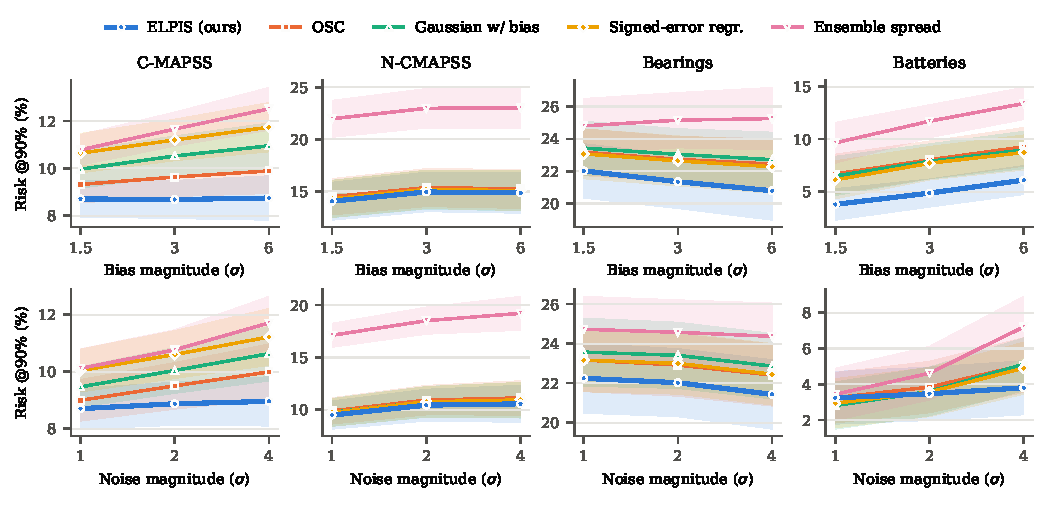
\includegraphics[width=\textwidth]{figures/severity.pdf}
\caption{Risk at 90\% coverage as fault severity grows (bias and noise magnitude in units of the channel's spread), seeds 72--81; bands are $\pm1.96$ standard errors of the mean absolute risk across pairs. Baselines as in Fig.~\ref{fig:rc}: Gaussian with learned bias~\cite{nix1994estimating}, signed-error regression~\cite{yoo2019learning}, ensemble spread~\cite{lakshminarayanan2017simple}.}
\label{fig:sev}
\end{figure}

\FloatBarrier
\section{Deployment analyses}\label{app:deploy}
\paragraph{Finite-sample certification on hard drives (post hoc).} Learn-then-Test~\cite{angelopoulos2021ltt} with the fixed-sequence procedure over coverage levels $0.05,\dots,1$, unit-level losses $b_u-r^\ast a_u$ and failure probability $\epsilon=0.1$ was applied to the 60 hard-drive deployments (seeds 92--121; 222 calibration units on the original drive models, 120 on the unseen ones), with $r^\ast$ a fraction $f\in\{1,0.85,0.7\}$ of the clean calibration units' accept-all optimistic rate. Hoeffding and Bernstein bounds certify nothing. The betting bound~\cite{waudbysmith2024betting} certifies $f=1$ at 95\% coverage in all 40 deployments with 222 units for \OSC, the Gaussian with learned bias and \AUTO{} (realised clean test risk 20.2--20.6\% against a target of 24.2--24.7\%, no violation; also no violation under the six faults, which on hard drives reduce optimism), $f=0.85$ in 4 of 40 (2 per seed set), $f=0.7$ in none, and nothing with 120 units. Plug-in thresholds without a bound exceed the target in 20--50\% of deployments. Guarantees are thus attainable with a few hundred labelled units, but only for weak targets; they do not distinguish the selectors.

\paragraph{Risk targets under unknown fault prevalence (post hoc).} On the round-4 runs (seeds 92--101, five families), we fixed thresholds on the calibration units and applied them unchanged to test mixtures in which a fraction $\pi\in\{0,0.1,0.3,0.5\}$ of windows carries one of the six unseen faults. For a risk target $r^\ast$ (half the accept-all optimistic rate of the clean calibration units), the plug-in rule takes the largest coverage at which the calibration risk is at most $r^\ast$. Two findings stand out. First, the realised risk of the one-sided selectors does not drift with fault prevalence. On C-MAPSS, \AUTO{} gives 5.36, 5.32, 5.24 and 5.16\% for $\pi=0,\dots,0.5$ (within 0.2 points on the other three benchmark families as well) (slightly above the mean target of 5.02\%) at nearly constant coverage (69.3, 69.1, 68.8 and 68.4\%; risk falls slightly with prevalence because faulty windows are rejected more often at the same threshold), whereas ensemble spread rises from 5.95 to 6.91\% and the Gaussian with learned bias from 5.05 to 5.90\%. At the same target, \AUTO{} keeps more coverage than \OSC: $+7.7$, $+8.9$ and $+31.7$ points on C-MAPSS, bearings and batteries (significant; Holm over 10), at a slightly larger excess over the target on C-MAPSS ($+0.55$ points). The battery gap is large because the target there is tiny (0.84\%): the largest admissible coverage is set by the top of the ranking, and small ranking differences move it in steps of 5 points. Second, a plug-in threshold is not a guarantee. On the four benchmark families \AUTO{} exceeds $r^\ast$ in 41--60\% of deployments, already without faults. With 4--26 calibration units the threshold is a point estimate, so it misses the target about half the time. Scores with fewer violations achieve them by accepting almost nothing. Adding perturbed copies to the calibration set (assumed prevalence 0.3) reduces the excess on C-MAPSS only slightly ($-0.22$ points, at 2.7 points of coverage). Adding the seen shifts instead is unsafe on hard drives, where it exceeds the target in every deployment.

\paragraph{Abstention versus a conservative offset (post hoc).} Could a conservative predictor replace abstention? We compared two policies, both fixed on the calibration units and aimed at $r^\ast$. The first, \emph{offset only}, shifts every prediction down by the smallest offset $b$ (in steps of $0.05\delta$) that meets $r^\ast$. The second, \emph{joint}, abstains at the 90\% calibration threshold of a score and then chooses the smallest offset that meets $r^\ast$ on the accepted windows. With clean calibration and $\pi=0.3$, the joint policy with \AUTO{} needs smaller offsets (0.00--1.10$\delta$ against 0.39--1.75$\delta$). It has both lower risk and lower RMSE than offset only on C-MAPSS, N-CMAPSS, batteries and hard drives; for example, on N-CMAPSS it reaches 6.88 against 8.89\% risk, with RMSE at 0.83 against 1.15 times that of the unshifted predictor. On bearings the two policies are close. When calibration includes perturbed copies (the pre-specified comparison), offset only must shift by up to $2.5\delta$. It then reaches lower risk on three families (by 1.1--3.2 points), but at an RMSE 16--232\% above the unshifted predictor, against $-6$ to $+17\%$ for the joint policy, whose RMSE is significantly lower on all five families (Holm over 10). Abstention therefore achieves safety at a much smaller cost in accuracy, but it complements a conservative offset rather than replacing it.




\FloatBarrier
\begin{footnotesize}
\bibliographystyle{unsrt}
\bibliography{refs}
\end{footnotesize}
\end{document}
